\clearpage
\appendix




\section{Related Works}
\label{sec:Appendix A}

\subsection{Federated learning with LoRA}
Recent studies have explored integrating LoRA into FL to alleviate the communication and computation overhead associated with fine-tuning large-scale models \cite{kuo2024federated, cho2024heterogeneous, fang2024automated, yi2023pfedlora}. 
FedIT \cite{zhang2024towards} is one of the earliest attempts to incorporate LoRA into FL, demonstrating that low-rank adapters can effectively reduce communication costs while maintaining competitive performance.
However, FedIT aggregates the two low-rank components in a straightforward manner and does not explicitly account for aggregation errors that arise during the aggregation process. 
To mitigate aggregation mismatch caused by heterogeneous client updates, several extensions have been proposed.
FLoRA \cite{wang2024flora} addresses heterogeneity and aggregation errors by stacking client-specific LoRA adapters at the server for aggregation.
FedEx-LoRA \cite{singhal2024fedex} alleviates aggregation error by introducing a residual correction term added to a fixed pre-trained weight matrix.
FlexLoRA \cite{bai2024federated} further addresses heterogeneity by reconstructing an ideal weight update matrix from the aggregated client adapters at the server, followed by singular value decomposition (SVD) to redistribute LoRA adapters with different ranks to individual clients.

\subsection{Differentially private federated LoRA}
More recent studies have investigated federated LoRA under differential privacy (DP) constraints.
FFA-LoRA \cite{sun2024improving} provides a detailed analysis of the noise amplification problem that arises when DP is applied to federated LoRA training, and mitigates this issue by updating only the $B$ component.
However, restricting updates to the $B$ component leads to a loss of expressiveness in LoRA.
To address this limitation, FedSVD \cite{lee2025fedsvd} similarly updates only the $B$ component, while leveraging orthogonalization and low-rank decomposition to alleviate the expressiveness loss and improve training stability under DP constraints.
Another line of work, which is most closely related to our study, aims to alleviate aggregation error by adopting alternating optimization strategies.
RoLoRA \cite{chen2025robust} and LoRA-A$^2$ \cite{koo2025towards} alternate the optimization of the two LoRA components across communication rounds, updating only one component at a time to reduce aggregation mismatch.
La-LoRA \cite{liu2026rethinking} further extend alternating optimization from communication rounds to local update steps.
While these methods empirically improve training stability, they rely on fixed and symmetric alternating schedules and do not explicitly account for the asymmetric roles of the two LoRA components during training.
In summary, existing federated LoRA-based approaches either restrict updates to a single component or adopt fixed, symmetric alternating schedules, both of which overlook the structural asymmetry between the two LoRA components and the round-wise dynamics of training. This motivates AS-LoRA, which makes principled, adaptive per-layer decisions based on training dynamics.

\newpage
% \FloatBarrier
\section{AS-LoRA Algorithm}
\label{sec:Appendix B}

\begin{figure}[h]
    \centering
    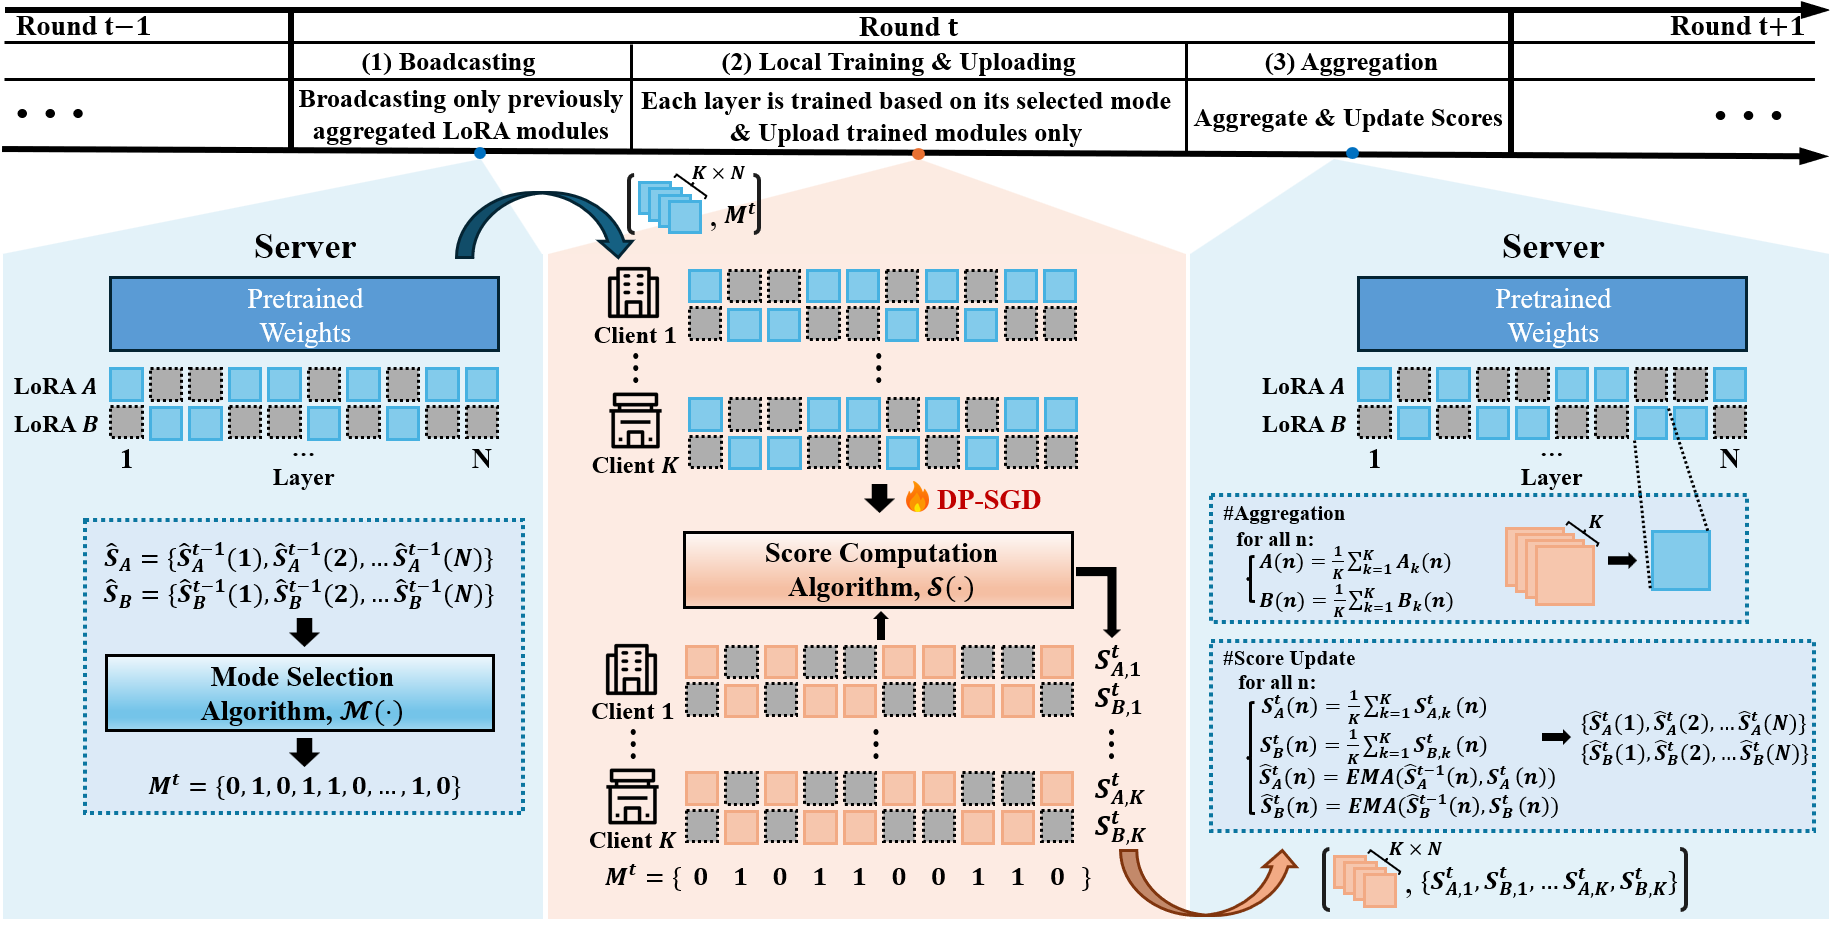
\includegraphics[width=1.0\textwidth]{./figures/8_appendix/AS-LoRA.png}
    \caption{Detail of the proposed AS-LoRA framework. }
    \label{fig:AS-LoRA_detail}
\end{figure}

\begin{figure}[h]
    \centering
    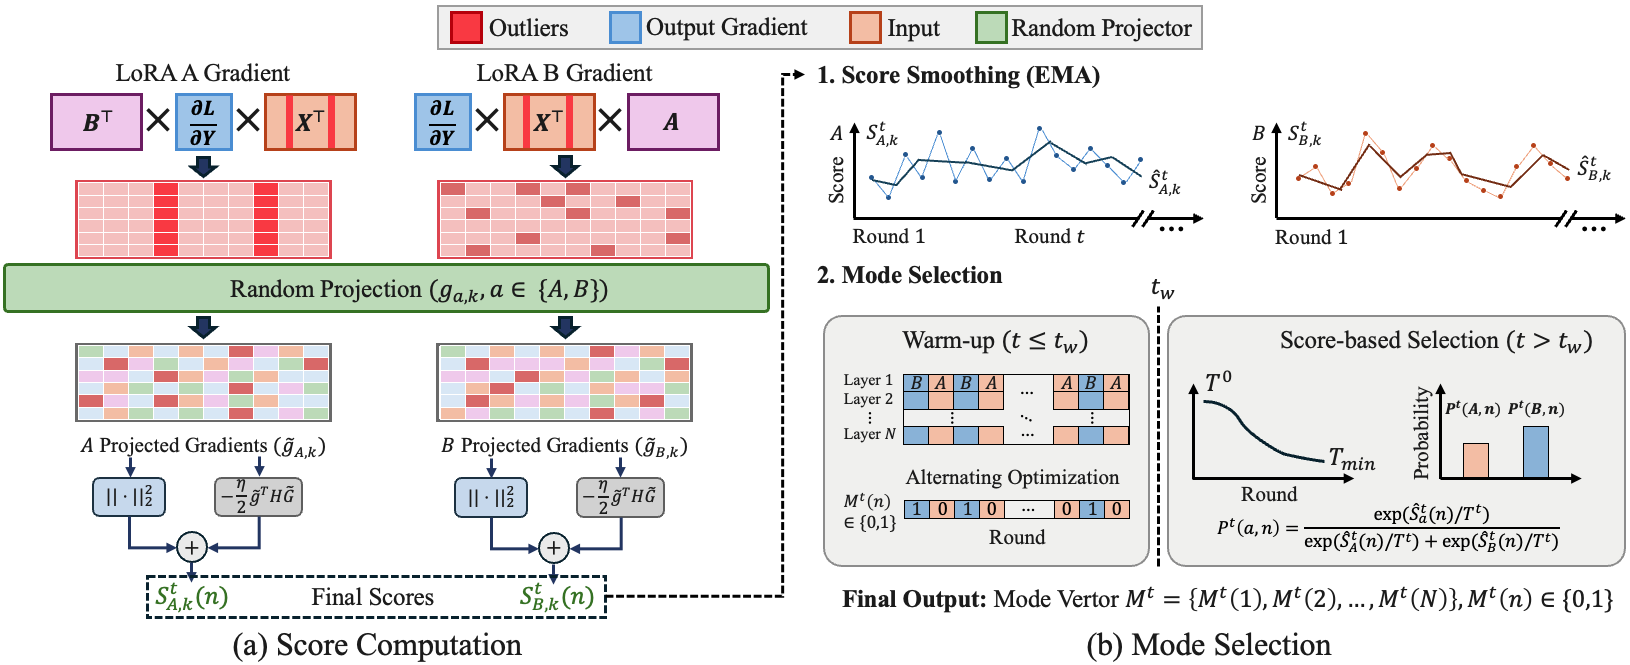
\includegraphics[width=1.0\textwidth]{./figures/8_appendix/random_projection_v2.png}
    \caption{ Detailed visualization of the proposed AS-LoRA score computation and mode selection procedures. (a) Component-wise scores are computed from the projected gradients of LoRA $A$ and $B$ matrices. Random projection mitigates the effect of channel-wise gradient outliers before applying the squared-gradient and curvature-aware score terms. (b) The server smooths the aggregated scores using EMA and performs layer-wise mode selection. During warm-up, AS-LoRA alternates between components, while after warm-up it uses a temperature-scaled score-based selection rule to produce the final mode vector. }
    \label{fig:score_mode_detail}
\end{figure}

\FloatBarrier
\begin{algorithm}[h]
\caption{AS-LoRA}
\label{alg:as_lora}
\begin{algorithmic}[1]

\STATE \textbf{Input:} communication rounds $T$, clients $K$, LoRA layers $N$
\STATE Initialize $A^0(n), B^0(n)$ and server scores 
$\hat{S}_A^{0}(n), \hat{S}_B^{0}(n)$ for all $n$

\FOR{$t=1$ \TO $T$}
    \STATE $M^t \leftarrow \mathcal{M}(\hat{S}_A^{t-1}, \hat{S}_B^{t-1})$
    
    \FOR{$k=1$ \TO $K$ \textbf{in parallel}}
        \STATE Update LoRA parameters using DP-SGD according to $M^t$
        \STATE Compute local scores 
        $S_{A,k}^t(n), S_{B,k}^t(n) \leftarrow \mathcal{S}(\cdot)$
        \STATE Upload updated parameters and scores to the server
    \ENDFOR

    \FOR{$n=1$ \TO $N$}
        \IF{$M^t(n)=0$}
            \STATE $A^t(n) \leftarrow \frac{1}{K}\sum_{k=1}^{K} A_k^t(n)$, 
            \quad $B^t(n) \leftarrow B^{t-1}(n)$
        \ELSE
            \STATE $B^t(n) \leftarrow \frac{1}{K}\sum_{k=1}^{K} B_k^t(n)$, 
            \quad $A^t(n) \leftarrow A^{t-1}(n)$
        \ENDIF

        \STATE $S_A^t(n) \leftarrow \frac{1}{K}\sum_{k=1}^{K} S_{A,k}^t(n)$, 
        \quad
        $S_B^t(n) \leftarrow \frac{1}{K}\sum_{k=1}^{K} S_{B,k}^t(n)$

        \STATE $\hat{S}_A^t(n) \leftarrow 
        \mathrm{EMA}\left(\hat{S}_A^{t-1}(n), S_A^t(n)\right)$,
        \quad
        $\hat{S}_B^t(n) \leftarrow 
        \mathrm{EMA}\left(\hat{S}_B^{t-1}(n), S_B^t(n)\right)$
    \ENDFOR
\ENDFOR

\STATE \textbf{Output:} final LoRA parameters $\{A^T(n), B^T(n)\}_{n=1}^{N}$

\end{algorithmic}
\end{algorithm}
%%%%%%%%%%%%%%%%%%%%%%%%%%%%%%%%%%%%%%%%%%%%%%%%%%%%%%%%%%%%%%%
\begin{algorithm}[h]
\caption{Score Computation $\mathcal{S}_{\|{g}\|^2}(\cdot)$ with Random Projection}
\label{alg:score_gnorm_rp}
\begin{algorithmic}[1]

\STATE \textbf{Input:} local loss $\mathcal{L}_k^t$, LoRA parameters $\{A_k^t(n), B_k^t(n)\}_{n=1}^{N}$, projection matrices $\{R_A(n), R_B(n)\}_{n=1}^{N}$
\STATE \textbf{Output:} local scores $\{S_{A,k}^t(n), S_{B,k}^t(n)\}_{n=1}^{N}$

\FOR{$n=1$ \TO $N$}
    \STATE Compute gradients:
    \[
    g_{A,k}^t(n) \leftarrow \nabla_{A_k^t(n)} \mathcal{L}_k^t,
    \quad
    g_{B,k}^t(n) \leftarrow \nabla_{B_k^t(n)} \mathcal{L}_k^t
    \]

    \STATE Apply Gaussian random projection:
    \[
    \widetilde{g}_{A,k}^t(n) \leftarrow g_{A,k}^t(n) R_A(n),
    \quad
    \widetilde{g}_{B,k}^t(n) \leftarrow R_B(n) g_{B,k}^t(n)
    \]

    \STATE Compute projected squared-gradient scores:
    \[
    S_{A,k}^t(n) \leftarrow \left\|\widetilde{g}_{A,k}^t(n)\right\|_2^2
    \]
    \[
    S_{B,k}^t(n) \leftarrow \left\|\widetilde{g}_{B,k}^t(n)\right\|_2^2
    \]
\ENDFOR

\RETURN $\{S_{A,k}^t(n), S_{B,k}^t(n)\}_{n=1}^{N}$

\end{algorithmic}
\end{algorithm}

\begin{algorithm}[h]
\caption{Score Computation $\mathcal{S}_{\mathrm{HVP}}(\cdot)$ with Random Projection}
\label{alg:score_hvp}
\begin{algorithmic}[1]

\STATE \textbf{Input:} local loss $\mathcal{L}_k^t$, LoRA parameters $\{A_k^t(n), B_k^t(n)\}_{n=1}^{N}$, projection matrices $\{R_A(n), R_B(n)\}_{n=1}^{N}$, learning rate $\eta$
\STATE \textbf{Output:} local scores $\{S_{A,k}^t(n), S_{B,k}^t(n)\}_{n=1}^{N}$

\FOR{$n=1$ \TO $N$}

    \STATE Compute gradients:
    \[
    g_{A,k}^t(n) \leftarrow \nabla_{A_k^t(n)} \mathcal{L}_k^t,
    \quad
    g_{B,k}^t(n) \leftarrow \nabla_{B_k^t(n)} \mathcal{L}_k^t
    \]

    \STATE Apply random projection:
    \[
    \widetilde{g}_{A,k}^t(n) \leftarrow g_{A,k}^t(n) R_A(n),
    \quad
    \widetilde{g}_{B,k}^t(n) \leftarrow R_B(n) g_{B,k}^t(n)
    \]

    \STATE Compute Hessian-vector products:
    \[
    h_{A,k}^t(n) \leftarrow H_{A(n)}(W_t)\,\widetilde{g}_{A,k}^t(n),
    \quad
    h_{B,k}^t(n) \leftarrow H_{B(n)}(W_t)\,\widetilde{g}_{B,k}^t(n)
    \]

    \STATE Compute scores:
    \[
    S_{A,k}^t(n) \leftarrow 
    \|\widetilde{g}_{A,k}^t(n)\|_2^2
    -
    \frac{\eta}{2}
    \widetilde{g}_{A,k}^t(n)^\top h_{A,k}^t(n)
    \]

    \[
    S_{B,k}^t(n) \leftarrow 
    \|\widetilde{g}_{B,k}^t(n)\|_2^2
    -
    \frac{\eta}{2}
    \widetilde{g}_{B,k}^t(n)^\top h_{B,k}^t(n)
    \]

\ENDFOR

\RETURN $\{S_{A,k}^t(n), S_{B,k}^t(n)\}_{n=1}^{N}$

\end{algorithmic}
\end{algorithm}

\begin{algorithm}[h]
\caption{Score Computation $\mathcal{S}_{\mathrm{FD}}(\cdot)$ with Random Projection}
\label{alg:score_fd}
\begin{algorithmic}[1]

\STATE \textbf{Input:} local loss $\mathcal{L}_k^t$, LoRA parameters $\{A_k^t(n), B_k^t(n)\}_{n=1}^{N}$, projection matrices $\{R_A(n), R_B(n)\}_{n=1}^{N}$, learning rate $\eta$, finite-difference radius $\epsilon_{\mathrm{fd}}$
\STATE \textbf{Output:} local scores $\{S_{A,k}^t(n), S_{B,k}^t(n)\}_{n=1}^{N}$

\FOR{$n=1$ \TO $N$}

    \STATE Compute gradients:
    \[
    g_{A,k}^t(n) \leftarrow \nabla_{A_k^t(n)} \mathcal{L}_k^t,
    \quad
    g_{B,k}^t(n) \leftarrow \nabla_{B_k^t(n)} \mathcal{L}_k^t
    \]

    \STATE Apply random projection:
    \[
    \widetilde{g}_{A,k}^t(n) \leftarrow g_{A,k}^t(n)R_A(n),
    \quad
    \widetilde{g}_{B,k}^t(n) \leftarrow R_B(n)g_{B,k}^t(n)
    \]

    \FOR{$a \in \{A,B\}$}

        \STATE Normalize the projected gradient direction:
        \[
        v_{a,k}^t(n) \leftarrow 
        \frac{\widetilde{g}_{a,k}^t(n)}
        {\|\widetilde{g}_{a,k}^t(n)\|_2+\epsilon}
        \]

        \STATE Estimate curvature by finite difference:
        \[
        c_{a,k}^t(n) \leftarrow
        \frac{
        \mathcal{L}_k^t\!\left(W_t+\epsilon_{\mathrm{fd}} v_{a,k}^t(n)\right)
        -2\mathcal{L}_k^t(W_t)
        +\mathcal{L}_k^t\!\left(W_t-\epsilon_{\mathrm{fd}} v_{a,k}^t(n)\right)
        }
        {\epsilon_{\mathrm{fd}}^2}
        \]

        \STATE Compute finite-difference score:
        \[
        S_{a,k}^t(n) \leftarrow
        \|\widetilde{g}_{a,k}^t(n)\|_2^2
        -
        \frac{\eta}{2}
        c_{a,k}^t(n)
        \|\widetilde{g}_{a,k}^t(n)\|_2^2
        \]

    \ENDFOR

\ENDFOR

\RETURN $\{S_{A,k}^t(n), S_{B,k}^t(n)\}_{n=1}^{N}$

\end{algorithmic}
\end{algorithm}
%%%%%%%%%%%%%%%%%%%%%%%%%%%%%%%%%%%%%%%%%%%%%%%%%%%%%%%%%
\begin{algorithm}[h]
\caption{Mode Selection $\mathcal{M}(\cdot)$ }
\label{alg:mode_selection}
\begin{algorithmic}[1]

\STATE \textbf{Input:} EMA scores $\{\hat{S}_A^t(n), \hat{S}_B^t(n)\}_{n=1}^{N}$, round $t$, warm-up period $t_w$, temperature parameters $(T^0, T_{\min}, \gamma)$
\STATE \textbf{Output:} mode vector $M^t = \{M^t(n)\}_{n=1}^{N}$

\IF{$t \le t_w$}
    \STATE \textbf{// warm-up: alternating schedule}
    \FOR{$n=1$ \TO $N$}
        \STATE $M^t(n) \leftarrow (t \bmod 2)$
    \ENDFOR

\ELSE
    \STATE Compute temperature:
    \[
    T^t \leftarrow \max\!\left(T_{\min},\, T^0 \cdot \gamma^{(t-t_w)}\right)
    \]

    \FOR{$n=1$ \TO $N$}

        \STATE Compute selection probabilities:
        \[
        P^t(A,n) \leftarrow 
        \frac{\exp\!\left(\hat{S}_A^t(n)/T^t\right)}
        {\exp\!\left(\hat{S}_A^t(n)/T^t\right) + \exp\!\left(\hat{S}_B^t(n)/T^t\right)}
        \]

        \STATE Sample mode:
        \[
        M^t(n) \sim \mathrm{Bernoulli}(P^t(A,n))
        \]

    \ENDFOR
\ENDIF

\RETURN $M^t$

\end{algorithmic}
\end{algorithm}
\FloatBarrier

\subsection{Visualization of AS-LoRA framework}
Fig~\ref{fig:AS-LoRA_detail} illustrates the overall workflow of the proposed AS-LoRA framework. 
At each communication round, the server first determines the layer-wise mode based on historical scores and broadcasts only the selected LoRA components. 
Each client then performs local updates using DP-SGD according to the assigned modes, computes component-wise scores, and uploads both the updated parameters and scores to the server. 
The server aggregates the selected components and updates the global scores, which are used for the next round of mode selection. 
This process enables adaptive, layer-wise optimization across communication rounds while mitigating aggregation error and unnecessary noise amplification. The overall training procedure of AS-LoRA is summarized in Algorithm~\ref{alg:as_lora}.

\subsection{Score Computation and Mode Selection}
Figure~\ref{fig:score_mode_detail} provides a detailed illustration of the score 
computation and mode selection procedures in AS-LoRA.

\textbf{Score Computation.}
Figure~\ref{fig:score_mode_detail}(a) depicts the score computation procedure 
performed on each client.
As illustrated, the gradient of LoRA-$A$ exhibits channel-wise outliers, where 
the gradient magnitude is highly concentrated in a small subset of channels.
To mitigate this, a Gaussian random projection is applied to each gradient, 
redistributing the concentrated magnitude across dimensions and enabling more 
reliable score estimation.
The score computation procedures with random projection are described in 
Algorithms~\ref{alg:score_gnorm_rp}--\ref{alg:score_fd}.

\textbf{Mode Selection.}
Figure~\ref{fig:score_mode_detail}(b) illustrates the mode selection procedure.
The server-side scores are smoothed via EMA to reduce round-to-round variance, 
and the mode for each layer is determined based on the smoothed scores.
During the warm-up phase ($t \leq t_w$), all layers follow a simple alternating 
schedule, where the $A$ and $B$ components are activated in alternation across 
rounds, and the mode vector $M^t(n) \in \{0, 1\}$ changes accordingly.
After the warm-up phase ($t > t_w$), score-based selection is activated.
The selection probability for each component is computed via a temperature-scaled 
softmax.

Here, the temperature $T^t$ follows an annealing schedule that decays from an 
initial value $T^0$ to a minimum $T_{\min}$ over training rounds.
This annealing encourages exploration of both components in early rounds while 
gradually shifting toward exploitation of the higher-scoring component as 
training progresses.
The final output is the mode vector
$M^t = \{M^t(1), M^t(2), \ldots, M^t(N)\}$, $M^t(n) \in \{0, 1\}$,
which specifies the active LoRA component for each layer at round $t$.
The full mode selection procedure is summarized in 
Algorithm~\ref{alg:mode_selection}.

\section{Preliminaries for Theoretical Analysis}
\label{app:prelim}


\subsection{Background}
We analyze AS-LoRA along two axes: \emph{(i) layer-wise freedom}---the ability to activate $A^{(n)}$ or $B^{(n)}$ independently per layer---and \emph{(ii) score-driven selection}---the greedy rule $\arg\max_{a\in\{A,B\}} S_a^{(n)}$ with $S_a^{(n)}=\|g_a^{(n)}\|^2-\tfrac{\eta}{2}(g_a^{(n)})^\top H_a^{(n)} g_a^{(n)}$. Each axis contributes a distinct and quantifiable advantage over the layer-tied or fixed-schedule baselines (FFA-LoRA~\citep{sun2024improving}, RoLoRA~\citep{chen2025robust}). The analysis combines block-coordinate descent theory~\cite{nesterov2012bcd}, Polyak--{\L}ojasiewicz convergence~\citep{karimi2016pl}, and DP-SGD privacy accounting~\citep{abadi2016deep,mironov2017renyi,wang2019sgm}.



\subsection{Setup}

Let $\Loss(W)=\tfrac{1}{K}\sum_{k=1}^K\Loss_k(W)$ be the federated loss over $K$ clients with per-client dataset size $m$ (total $Km$ samples). For layer $n\in[N]$, the frozen weight is $W_0^{(n)}\in\R^{d\times d}$ and the LoRA update factorizes as $B^{(n)}A^{(n)}$ with $B^{(n)}\in\R^{d\times r}$, $A^{(n)}\in\R^{r\times d}$, and rank $r\!\ll\!d$, so that the effective weight is $W^{(n)}=W_0^{(n)}+B^{(n)}A^{(n)}$ acting on an input $X\in\R^{d\times m}$ as $W^{(n)}X^{(n)}=W_0^{(n)}X+B^{(n)}A^{(n)}X^{(n)}$

\paragraph{Stochastic gradient and population Hessian.}
For each block label $a\in\{A,B\}$, let $g_a^{(n)}$ denote the \emph{mini-batch stochastic gradient} of $\Loss$ with respect to the factor matrix $a^{(n)}$, satisfying $\E[g_a^{(n)}]=\nabla_{a^{(n)}}\Loss$ over the random sampling. Concretely, $g_A^{(n)}\in\R^{r\times d}$ and $g_B^{(n)}\in\R^{d\times r}$ are matrix-valued. The corresponding \emph{deterministic population Hessian} $H_a^{(n)}(W):=\nabla^2_{a^{(n)}}\Loss(W)$ acts on the vectorized factor and is treated as a $(\dim a^{(n)})\!\times\!(\dim a^{(n)})$ matrix throughout (with $\dim A^{(n)}=\dim B^{(n)}=rd$). Randomness enters only through $g_a^{(n)}$ and DP-SGD noise $\Gauss_a\!\sim\!\Gauss(0,\sigma^2 C^2 I)$ (clipping bound $C$), and $\nabla_{a^{(n)}}\Loss$ and $H_a^{(n)}(W)$ are deterministic functions of $W$ as in the standard convention for second-order SGD/BCD analyses~\cite{karimi2016pl,nesterov2012bcd}. With $\|\cdot\|$ denoting the Frobenius norm for matrices and the Euclidean norm for vector objects, the per-layer block Rayleigh quotient is $\lambda_a^{(n)}:=\langle g_a^{(n)}, H_a^{(n)} g_a^{(n)}\rangle/\|g_a^{(n)}\|^2$ and the per-layer block-greedy score is $S_a^{(n)}:=\|g_a^{(n)}\|^2-\tfrac{\eta}{2}\langle g_a^{(n)}, H_a^{(n)} g_a^{(n)}\rangle$. 

\begin{remark}[Practical estimation of $H_a^{(n)} g_a^{(n)}$]\label{rem:hvp}
All theoretical statements use the population Hessian $H_a^{(n)}(W)=\nabla^2_{a^{(n)}}\Loss(W)$. In practice, the curvature term $\langle g_a^{(n)}, H_a^{(n)} g_a^{(n)}\rangle$ is computed via a single Hessian-vector product on the same mini-batch used for $g_a^{(n)}$ (Pearlmutter trick) or via a Hutchinson-style sketch~\citep{yao2020pyhessian}; the resulting estimation bias is $O(\sigma_g^2/m)$ and is absorbed into the $\eta\beta\sigma_g^2$ noise term of Theorem~\ref{thm:conv} without altering any rate.
\end{remark}

\paragraph{Moore--Penrose pseudoinverse and orthogonal projectors.}
Several reconstruction-floor and subspace-misalignment quantities are stated in terms of the Moore--Penrose pseudoinverse, which we briefly recall. For any matrix $M\in\R^{p\times q}$, the \emph{Moore--Penrose pseudoinverse} $M^\dagger\in\R^{q\times p}$ is the unique matrix satisfying the four Penrose conditions $M M^\dagger M = M$, $M^\dagger M M^\dagger = M^\dagger$, $(M M^\dagger)^\top = M M^\dagger$, $(M^\dagger M)^\top = M^\dagger M$~\citep{penrose1955}. Three properties are used repeatedly. (i) When $M$ is square and invertible, $M^\dagger = M^{-1}$. (ii) When $M$ is row full-rank (the generic case for our LoRA factors $A^t(n)\in\R^{r\times d}$ with $r<d$), $M^\dagger = M^\top(MM^\top)^{-1}$, and $A^t(n)\,A^t(n)^\dagger = I_r$ acts as a right inverse. (iii) The two products $M M^\dagger\in\R^{p\times p}$ and $M^\dagger M\in\R^{q\times q}$ are precisely the orthogonal projectors onto $\mathrm{col}(M)\subseteq\R^p$ and $\mathrm{row}(M)\subseteq\R^q$ respectively. Operationally, the least-squares minimum-norm solution of $Mx=b$ is $x^\star = M^\dagger b$, which is the property used to obtain the closed-form FFA-LoRA minimizer in the proof of Theorem~\ref{thm:irreducible}. All projectors $P_{A^t(n)}=A^t(n)^\dagger A^t(n)$ used in the analysis are of form (iii) and project onto the row-span of the corresponding factor matrix.



\subsection{Assumptions}
First, we collect here all assumptions invoked by the main text. Assumptions~\ref{asm:smooth}--\ref{asm:pl} are the standard block / per-layer counterparts of the smoothness, bounded-variance, Hessian-spectrum, and Polyak--{\L}ojasiewicz (PL) conditions used in modern SGD/BCD/PL analyses~\cite{nesterov2012bcd,karimi2016pl}. Strong convexity of the Assumption \ref{asm:hess} is invoked only on the per-layer reconstruction quadratic, not on the full non-convex loss, and the PL condition of Assumption \ref{asm:pl} replaces it for end-to-end statements.

\begin{assumption}[Block smoothness]\label{asm:smooth}
Each $\Loss_k$ is $L$-smooth and block-smooth with constants $L_A^{(n)},L_B^{(n)}$, and $\beta:=\max_{a,n}L_a^{(n)}$.
\end{assumption}
\begin{assumption}[Bounded stochastic variance]\label{asm:var}
$\E\|g_a^{(n)}-\nabla_{a(n)}\Loss\|^2\le\sigma_g^2$ for every layer $n$ and block label $a\in\{A,B\}$, and per-sample clipping $\|g_{a,i}^{(n)}\|\le C$ a.s.
\end{assumption}
\begin{assumption}[Block strong convexity and Lipschitz Hessian]\label{asm:hess}
$\mu_a^{(n)}I\preceq H_a^{(n)}\preceq L_a^{(n)} I$, and $H$ is $L_H$-Lipschitz.
\end{assumption}
\begin{assumption}[PL condition, non-convex]\label{asm:pl}
$\|\nabla\Loss\|^2\ge 2\mu(\Loss-\Loss^\star)$ for some $\mu>0$~\citep{karimi2016pl}.
\end{assumption}





\subsection{Mathematical Preliminaries}


This appendix collects the standard tools from matrix analysis \cite{horn2012matrix}, high-dimensional probability \cite{vershynin2018}, and convex optimization \cite{nesterov2018book}.

\begin{lemma}[Norm submultiplicativity and SVD-based reverse bound]\label{lem:norm-sandwich}
For any $M\in\R^{p\times d}$ and $X\in\R^{d\times m}$ of compatible dimensions (so that $MX\in\R^{p\times m}$ is well defined),
\begin{equation}
\|MX\|_F \;\le\; \sigma_{\max}(X)\,\|M\|_F,
\end{equation}
where $\sigma_{\max}(X)=\|X\|_\text{op}$ is the largest singular value of $X$. We refer to this as the standard inequality. If the rows of $M$ lie in $\mathrm{col}(X^\top)=\mathrm{row}(X)$, equivalently $M=M\,P_{X}$ where $P_X=X^\top(XX^\top)^{-1}X$ when $X$ has full row rank, then the matching reverse inequality holds:
\begin{equation}
\|MX\|_F \;\ge\; \sigma_{\min}^+(X)\,\|M\|_F,
\end{equation}
with $\sigma_{\min}^+(X)$ the smallest \emph{nonzero} singular value of $X$.
\end{lemma}
\begin{proof}

The upper bound is directly from \cite{horn2012matrix}. For the proof of lower bound, let $X=U\Sigma V^\top$ be the SVD with $\Sigma=\mathrm{diag}(\sigma_1,\ldots,\sigma_k,0,\ldots,0)$, $\sigma_1\ge\cdots\ge\sigma_k>0$, $k=\mathrm{rank}(X)$. Then $\|MX\|_F^2=\|MU\Sigma V^\top\|_F^2=\|MU\Sigma\|_F^2$ (Frobenius is invariant under right multiplication by orthogonal $V^\top$). Writing $MU=:N$ with columns $n_1,\ldots,n_d$, $\|MU\Sigma\|_F^2=\sum_{i=1}^d\sigma_i^2\|n_i\|^2$. If rows of $M$ lie in $\mathrm{row}(X)$, then $n_i=0$ for all $i>k$, so $\sum_i\sigma_i^2\|n_i\|^2\ge\sigma_k^2\sum_{i\le k}\|n_i\|^2=(\sigma_{\min}^+(X))^2\|M\|_F^2$.
\end{proof}


\begin{lemma}[High-probability bound of covariance estimation \cite{vershynin2018}, Rem.~4.7.3]\label{lem:cov-conc}
Let $x_1,\ldots,x_n\in\R^d$ be i.i.d.\ zero-mean random vectors with population covariance $\Sigma:=\E[x_ix_i^\top]$, satisfying 
\begin{equation}\label{cond_shapeaware}
\bigl\|\langle X,v\rangle\bigr\|_{\psi_2} \;\le\; \kappa\,\bigl\|\langle X,v\rangle\bigr\|_{L^2} \qquad\text{for every } v\in\R^d,
\end{equation}
with parameter $\kappa$. Then for every $u\ge 0$, with probability at least $1-2e^{-u}$,
\begin{equation}
\Bigl\|\tfrac{1}{n}\!\sum_{i=1}^n\! x_ix_i^\top - \Sigma\Bigr\|_\text{op} \;\le\; C\,\kappa^2\,\|\Sigma\|_\text{op}\!\Bigl(\sqrt{(d+u)/n}+(d+u)/n\Bigr),
\end{equation}
for an absolute constant $C>0$. In particular, for $n\gtrsim d$ and any fixed confidence level $1-2e^{-u}$,
\begin{equation}
\bigl\|\tfrac{1}{n}\!\sum_{i=1}^n\! x_ix_i^\top - \Sigma\bigr\|_\text{op} \;=\; O_p\!\bigl(\kappa^2\|\Sigma\|_\text{op}\sqrt{d/n}\bigr).
\end{equation}
\end{lemma}


%\begin{lemma}[Davis--Kahan for spectral projections \cite{vershynin2018}, Exercise 4.13]\label{lem:davis-kahan}
%Let $\widehat\Sigma,\Sigma\in\R^{d\times d}$ be symmetric and let $V_r,\widehat V_r\in\R^{d\times r}$ have orthonormal columns spanning the top-$r$ eigenspaces of $\Sigma,\widehat\Sigma$ respectively. Suppose $\Sigma$ has eigengap $\Delta:=\lambda_r(\Sigma)-\lambda_{r+1}(\Sigma)>0$. Then the orthogonal projectors $P:=V_rV_r^\top$ and $\widehat P:=\widehat V_r\widehat V_r^\top$ satisfy
%\begin{equation}
%\|\widehat P - P\|_\text{op} \;\le\; \frac{2\,\|\widehat\Sigma-\Sigma\|_\text{op}}{\Delta}.
%\end{equation}
%\end{lemma}

\begin{lemma}[Linear convergence of GD on strongly-convex smooth functions \cite{nesterov2018book}, Thm. 2.3.4]\label{lem:contract}
Let $f:\R^{p\times q}\to\R$ be twice differentiable with Hessian satisfying $\mu I\preceq\nabla^2 f\preceq L I$ for $0<\mu\le L$. Let $X^\star=\arg\min f$. Then gradient descent $X_{t+1}=X_t-\eta\nabla f(X_t)$ with step size $\eta\le 1/L$ satisfies
\begin{equation}
\|X_{t+1}-X^\star\|_F^2 \;\le\; (1-\eta\mu)\,\|X_t-X^\star\|_F^2 \;\le\; (1-\mu/L)\,\|X_t-X^\star\|_F^2.
\end{equation}
\end{lemma}


\begin{lemma}[Second-order Taylor with cubic remainder \cite{nesterov2018book}, Lemma 1.2.4]\label{lem:taylor}
Let $\Loss:\R^d\to\R$ be twice differentiable with $L_H$-Lipschitz Hessian: $\|\nabla^2\Loss(x)-\nabla^2\Loss(y)\|_\text{op}\le L_H\|x-y\|$. Then for any $W,h$,
\begin{equation}
\Bigl|\Loss(W+h)-\Loss(W)-\langle\nabla\Loss(W),h\rangle-\tfrac12 h^\top\nabla^2\Loss(W)h\Bigr| \;\le\; \tfrac{L_H}{6}\|h\|^3.
\end{equation}
\end{lemma}










\section{Proof of Theorem \ref{thm:privacy}}
\label{app:proof_of_privacy}
The DP-SGD mechanism of \cite{abadi2016deep} uses subsampled Gaussian noise: at each round, sample a fraction $q$ of clients, compute clipped gradients $\tilde g_i=\Pi_{\|\cdot\|\le C}(g_i)$, aggregate $\bar g=\sum_{i\in\text{batch}}\tilde g_i+\Gauss(0,\sigma^2 C^2 I)$. By the moments accountant / R\'enyi-DP analysis of \cite{mironov2017renyi,wang2019sgm}, each round contributes at most $\tfrac{q^2C^2}{\sigma^2}$ to the cumulative R\'enyi-DP $(\alpha,\epsilon_\alpha)$ budget at order $\alpha$. R\'enyi-DP composes additively. $T$ rounds give cumulative R\'enyi-DP cost at most $T\cdot q^2C^2/\sigma^2$ at order $\alpha$. Converting to $(\epsilon,\delta)$-DP via the standard tail bound $\epsilon=\epsilon_\alpha+\log(1/\delta)/(\alpha-1)$ and optimising over $\alpha$ yields $\epsilon\le q^2 C^2 T\log(1/\delta)/\sigma^2$. The AS-LoRA selection $\arg\max_{a\in\{A,B\}}S_a^{(n),t}$ uses the per-block scores $S_a^{(n),t}=\|\bar g_a^{(n)}\|^2-\tfrac{\eta}{2}\langle \bar g_a^{(n)}, H_a^{(n)}\bar g_a^{(n)}\rangle$, where $\bar g_a^{(n)}$ is the already-clipped, already-noised, before being aggregated. Since $H_a^{(n)}$ is also computed on the same mini-batch, the score is a deterministic function of $\bar g_a^{(n)}$. The post-processing invariance of differential privacy~\cite{dwork2014dpfoundations} says that \emph{any function applied to the output of an $(\epsilon,\delta)$-DP mechanism remains $(\epsilon,\delta)$-DP}. Since $M^t(n)$ is computed deterministically from $\{\bar g_a^{(n)}\}_{a,n}$, which are already DP-protected, no additional privacy cost is incurred. The total AS-LoRA privacy ledger therefore matches FFA-LoRA / RoLoRA exactly. \hfill$\square$




\section{Proof of Theorem \ref{thm:irreducible}}
\label{app:proof_of_irreducible}
Fix layer $n$. Under FFA-LoRA, $A^{(n)}$ is permanently fixed at $A^0(n)$ and only $B^{(n)}$ is updated by SGD with step size $\eta$. Because the per-layer reconstruction loss is convex quadratic in $B^{(n)}$ (when $A^{(n)}$, $X_n$ are fixed), standard SGD theory on convex quadratics guarantees that the iterates $B^{(n)}_t$ converge in expectation to the static minimizer $B_\text{FFA}(n)$ of
\begin{equation}
\ell^{(n)}(B) \;=\; \tfrac12\bigl\|B^\star(n)A^\star(n) X_n - B\,A^0(n) X_n\bigr\|_F^2,
\end{equation}
up to an $O(\eta\sigma_g^2)$ noise floor \cite{bottou2018sgd}. Consequently,
\begin{equation}
\lim_{T\to\infty}\E[\mathcal R_\text{rec}^{(n),\text{FFA}}] \;=\; \min_B\ell^{(n)}(B)/(Km) \;+\; O(\eta\sigma_g^2),
\end{equation}
and the first term is fully determined by the static least-squares minimization. The $O(\eta\sigma_g^2)$ correction is a standard SGD noise-floor term, not a function of the misalignment $\delta^0(n)$, so it does not affect the qualitative shape of the floor. We absorb it into $\tilde c$ for the remainder of the proof. The function $\ell^{(n)}(B)$ is convex quadratic in $B$ with Hessian $A^0(n)X_n X_n^\top A^0(n)^\top\otimes I$, which is positive definite when $A^0(n)X_n$ has full row rank (the generic case). Setting $\nabla_B\ell^{(n)}(B)=0$ gives the normal equation
\begin{equation}
\bigl(B\,A^0(n) X_n - B^\star(n) A^\star(n) X_n\bigr)\,(A^0(n) X_n)^\top \;=\; 0,
\end{equation}
which solves to
\begin{equation}
B_\text{FFA}(n) \;=\; B^\star(n)A^\star(n)\,X_n X_n^\top A^0(n)^\top \bigl(A^0(n)\,X_n X_n^\top A^0(n)^\top\bigr)^{-1}.
\end{equation}
This is the matrix Moore--Penrose form of the least-squares solution: writing $Z=A^0(n)X_n$, the optimal $B$ is precisely $B^\star A^\star X_n\cdot Z^\dagger$. Recall $Z^\dagger=Z^\top(ZZ^\top)^{-1}$ for row full-rank $Z$. Substituting back,
\begin{equation}
\min_B \ell^{(n)}(B) \;=\; \tfrac12\bigl\|B^\star(n)A^\star(n)\,X_n\,(I_m-P^\text{row}_{A^0(n) X_n})\bigr\|_F^2,
\end{equation}
where
\begin{equation}\label{row_projector}
P^\text{row}_{A^0(n)X_n} \;:=\; X_n^\top A^0(n)^\top \bigl(A^0(n)\,X_n X_n^\top A^0(n)^\top\bigr)^{-1} A^0(n)\,X_n \;\in\;\R^{m\times m}
\end{equation}
is the orthogonal projector onto $\mathrm{row}(A^0(n)X_n)$ inside $\R^m$ (the sample-index space), confirming that $B^\star(n)A^\star(n)\,X_n\,(I_m-P^\text{row}_{A^0(n) X_n})$ is the part of $B^\star A^\star X_n$ orthogonal to $\mathrm{row}(A^0(n)X_n)$.Bring the residual into the parameter space via the trace identity
\begin{equation} \label{residual}
\bigl\|B^\star A^\star X_n(I-P^\text{row}_{A^0(n)X_n})\bigr\|_F^2 =\tr\bigl((B^\star A^\star)\,M_n\,(B^\star A^\star)^\top\bigr),\quad M_n := X_n(I-P^\text{row}_{A^0(n)X_n})X_n^\top.
\end{equation} 
Setting $S := X_n X_n^\top$ and expanding $P^\text{row}_{A^0(n)X_n}$ explicitly, $M_n$ admits the \emph{Schur complement representation}
\begin{equation} \label{M_n}
M_n \;=\; S - S\,A^0(n)^\top\bigl(A^0(n)\,S\,A^0(n)^\top\bigr)^{-1}\,A^0(n)\,S.
\end{equation}

We assume the per-layer input distribution $\mathcal D_X^{(n)}$ produces zero-mean random vectors $x\sim\mathcal D_X^{(n)}$ satisfying the shape-aware sub-Gaussian condition \eqref{cond_shapeaware} in Lemma \ref{lem:cov-conc} with parameter $\kappa^{(n)}=O(1)$ uniformly across layers and clients, which is the standard condition in or sample-covariance concentration in operator norm \cite{vershynin2018}. In specific, it is satisfied by Gaussian and log-concave distributions \cite{vershynin2018}. Throughout we treat $\kappa^{(n)}$, $\|\Sigma_X^{(n)}\|_\text{op}$, and $\|B^\star A^\star\|_\text{op}$ as $\Theta(1)$ constants in the rate notation. 


Lemma~\ref{lem:cov-conc} gives $S/(Km) = \Sigma_X^{(n)} + O_p(1/\sqrt{Km})$, which under the well-conditioned input regime propagates through the Schur complement to
\begin{equation} \label{M_n_2}
M_n/(Km) =\Sigma_X^\perp \;+\; O_p(1/\sqrt{Km}), \qquad \Sigma_X^\perp :=\Sigma_X^{(n)} - \Sigma_X^{(n)} A^0(n)^\top\bigl(A^0(n)\Sigma_X^{(n)} A^0(n)^\top\bigr)^{-1} A^0(n)\,\Sigma_X^{(n)}.
\end{equation}
Here, the Schur complement $\Sigma_X^\perp\in\R^{d\times d}$ has kernel $\mathrm{row}(A^0(n))$, which can be easily derived. We have 
\begin{equation} \label{correction}
\tfrac{1}{Km}\,\|B^\star A^\star X_n(I-P^\text{row}_{A^0(n)X_n})\|_F^2 \;=\; \tr\bigl((B^\star A^\star)\,\Sigma_X^\perp\,(B^\star A^\star)^\top\bigr) \;+\; O_p(1/\sqrt{Km}),
\end{equation}
by combining \eqref{residual}--\eqref{M_n_2}.
Because $\Sigma_X^\perp$ has kernel $\mathrm{row}(A^0(n))$, only the part of $B^\star A^\star$ outside $\mathrm{row}(A^0(n))$ contributes, \emph{i.e.} $B^\star A^\star(I-P_{A^0(n)})$. Now, we apply Lemma~\ref{lem:norm-sandwich} to
\begin{equation}
\tr\bigl((B^\star A^\star)\,\Sigma_X^\perp\,(B^\star A^\star)^\top\bigr)= \|B^\star A^\star (\Sigma_X^\perp)^{1/2}\|_F^2=
\|B^\star A^\star(I-P_{A^0(n)}) (\Sigma_X^\perp)^{1/2}\|_F^2
\end{equation}
with $M= B^\star A^\star(I-P_{A^0(n)})$ and $X = (\Sigma_X^\perp)^{1/2}$ and obtain
\begin{equation}
\lambda_{\min}^+(\Sigma_X^\perp)\,(\delta^0(n))^2 \;\le\; \tr\bigl((B^\star A^\star)\,\Sigma_X^\perp\,(B^\star A^\star)^\top\bigr) \;\le\; \lambda_{\max}(\Sigma_X^\perp)\,(\delta^0(n))^2,
\end{equation}
where $\lambda_{\min}^+(\Sigma_X^\perp) > 0$ is the smallest nonzero eigenvalue (acting on $\ker A^0(n)$) and $\lambda_{\max}(\Sigma_X^\perp) \le \|\Sigma_X^{(n)}\|_\text{op} = O(1)$. Under the well-conditioned input regime, both eigenvalue bounds are $\Theta(1)$, so the sandwich's two endpoints have the same order $\Theta((\delta^0(n))^2)$. Combined with the $O_p(1/\sqrt{Km})$ correction \eqref{correction}, we have
\begin{equation}
    \min_B \ell^{(n)}(B)\cdot\tfrac{1}{Km} \;=\; \Theta\bigl((\delta^0(n))^2\bigr).
\end{equation}
Because $\mathcal R_\text{rec}$ is layer-additive \emph{by definition}, summing the per-layer $\Theta$ statements and dividing by $N$ gives, with no further independence assumption,
\begin{equation}
\lim_{T\to\infty}\E\bigl[\mathcal R_\text{rec}(\mathbf W_T^\text{FFA})\bigr] \;=\; \Theta\!\Bigl(\tfrac{1}{N}\sum_n (\delta^0(n))^2\Bigr),    
\end{equation}
the implicit constant absorbing the per-layer conditioning $\sigma_{\max}^2(X_n)/\sigma_{\min}^2(X_n A^0(n)^\dagger)$, the correction $O_p(1/\sqrt{Km})$, and any SGD noise floor $O(\eta\sigma_g^2)$. 

\emph{RoLoRA lower bound via pigeonhole.} For any layer-tied schedule $M^t\in\{\mathbf 1_A,\mathbf 1_B\}$ with $A$-active set $\mathcal R_A:=\{t\le T:M^t=\mathbf 1_A\}$ of size $|\mathcal R_A|=\lfloor T/2\rfloor$, consider an adversarial layer configuration where the per-layer \emph{optimal $A$-active sets} $\mathcal S_1,\ldots,\mathcal S_N\subseteq[T]$ partition $[T]$ into $N$ equal parts of size $T/N$ each (assuming $N\mid T$ for clarity; the general case differs by $O(1)$). Define the \emph{mismatch set for layer $n$} as $\mathcal S_n\setminus\mathcal R_A$, which are the rounds where layer $n$'s optimal protocol calls for $A$-active but the schedule has $B$ active globally, so $A^t(n)$ remains unchanged and $\delta^t(n)$ cannot contract on these rounds.

Since $\{\mathcal S_n\}$ partition $[T]$,
\begin{equation}
\sum_{n=1}^N |\mathcal R_A\cap\mathcal S_n| \;=\; |\mathcal R_A| \;=\; T/2,
\end{equation}
so by averaging, at least one layer $n^\star$ has $|\mathcal R_A\cap\mathcal S_{n^\star}|\le T/(2N)$. The mismatch count for this layer is
\begin{equation}
|\mathcal S_{n^\star}\setminus\mathcal R_A| \;=\; |\mathcal S_{n^\star}| - |\mathcal R_A\cap\mathcal S_{n^\star}| \;\ge\; T/N - T/(2N) \;=\; T/(2N) \;=\; \Omega(T).
\end{equation}
On each mismatch round, $M^t = \mathbf 1_B$ so $A^t(n^\star)$ is unchanged; the contracting (matched) rounds for layer $n^\star$ are at most $T/(2N)$, half of what AS-LoRA-style adaptive selection could achieve. In the regime where this bounded number of contractions is insufficient to drive $\delta$ to zero (e.g., finite-$T$ analysis or contraction ratio close to $1$), $\delta^T(n^\star)\ge(1-\epsilon)\,\delta^0(n^\star)$ persists for some $\epsilon\in(0,1)$. Plugging into the per-layer $\Theta$ floor yields
\begin{equation}
\E\bigl[\mathcal R_\text{rec}(\mathbf W_T^\text{RoLoRA})\bigr] \;=\; \Omega\!\Bigl(\tfrac{1}{N}\sum_n (\delta^0(n))^2\Bigr),
\end{equation}
matching the FFA $\Theta$ floor up to the multiplicative factor $(1-\epsilon)^2\in(0,1]$. \hfill$\square$



\section{Proof of Corollary~\ref{cor:asstrict}}
\label{app:proof-asstrict}

Fix layer $n$ and consider a round $t$ at which AS-LoRA activates the down-projection block $A^{(n)}$. Recall $\delta^t(n) = \|B^\star(n)A^\star(n)(I-P_{A^t(n)})\|_F$. The per-layer reconstruction loss $\ell^{(n)}(A,B) = \tfrac12\|B^\star A^\star X_n - BA X_n\|_F^2$, viewed as a function of $A$ alone (with $B$ fixed at any value achieving the layer-$n$ optimum given $A$), is convex quadratic in $A$ with Hessian sandwich $\mu_A^{(n)} I\preceq H_A^{(n)}\preceq L_A^{(n)} I$ (Assumptions~\ref{asm:smooth}, \ref{asm:hess}). Applying Lemma~\ref{lem:contract} with step size $\eta\le 1/L_A^{(n)}$ yields
\begin{equation} \label{cor_1}
\|A^{t+1}(n)-A_\text{opt}(n)\|_F^2 \;\le\; \bigl(1-\mu_A^{(n)}/L_A^{(n)}\bigr)\,\|A^t(n)-A_\text{opt}(n)\|_F^2,
\end{equation}
where $A_\text{opt}(n)$ is the local minimizer at layer $n$ and a particular gauge representative of $A^\star(n)$. As we have seen in the proof of Theorem \ref{thm:irreducible}, the map $A\mapsto P_A=A^\dagger A$ is locally Lipschitz on the manifold of full-row-rank matrices. By Davis--Kahn--Wedin sin$\Theta$ theorem \citep{wedin1972}, for $A,\widetilde A\in\R^{r\times d}$ both row-full-rank with smallest singular values bounded below by $\sigma>0$,
\begin{equation}
\bigl\|P_A - P_{\widetilde A}\bigr\|_F \; = \; \sqrt{2}\bigl\|\mathrm{sin}\Theta \bigr\|_F \;\le\; \frac{C}{\sigma}\,\bigl\|A-\widetilde A\bigr\|_F
\end{equation}
for an absolute constant $C$. Applying with $A=A^{t+1}(n)$, $\widetilde A=A_\text{opt}(n)$, and $\sigma=\sigma_{\min}(A_\text{opt}(n))$ gives
\begin{equation}\label{cor_2}
\|P_{A^{t+1}(n)}-P_{A_\text{opt}(n)}\|_F \;\le\; \frac{C}{\sigma_{\min}(A_\text{opt}(n))}\,\|A^{t+1}(n)-A_\text{opt}(n)\|_F.
\end{equation}

Using the fact that $B^\star A^\star (I-P_{A_\text{opt}})=0$ ($\mathrm{ker}(A^{\star})=\mathrm{ker}(A_{\mathrm{opt}})$), we have $\delta^t(n)=\|B^\star A^\star(P_{A_\text{opt}}-P_{A^t})\|_F$, so
\begin{equation}
\delta^{t+1}(n) \;\le\; \|B^\star A^\star\|_\text{op}\,\|P_{A_\text{opt}}-P_{A^{t+1}}\|_F.
\end{equation}
Combining \eqref{cor_1} and \eqref{cor_2}, using $\|B^\star A^\star\|_\text{op}=\Theta(1)$, $\sigma_{\min}(A_\text{opt})=\Theta(1)$ under the assumption and discussion with Theorem \ref{thm:irreducible}, one obtains the per-layer geometric contraction
\begin{equation} \label{geometric_cont}
\delta^{t+1}(n) \;\le\; \sqrt{1-\mu_A^{(n)}/L_A^{(n)}}\cdot\delta^t(n) \;=:\; \gamma_n\cdot\delta^t(n), \qquad \gamma_n\in(0,1).
\end{equation}
On rounds where $M^t(n)=B$ instead, $A^{(n)}$ is unchanged, so $P_{A^t(n)}$ and hence $\delta^t(n)$ are unchanged. Thus $\delta^t(n)$ is monotonically non-increasing across the trajectory, and contracts strictly only on $A$-active rounds.

By the hypothesis of the corollary, there exists $c\in(0,1)$ such that $|\{t\le T:M^t(n)=A\}|\ge cT$ for every $n$ (with probability one for argmax, in expectation for softmax). Combining with \eqref{geometric_cont}, we have 
\begin{equation}
\delta^T(n) \;\le\; \gamma_n^{cT}\cdot\delta^0(n).
\end{equation}
This is the geometric-decay form, where every $A$-active round multiplies $\delta$ by at most $\gamma_n<1$, and we have at least $cT$ such rounds. Solve $\gamma_n^{cT}\delta^0(n)\le\varepsilon$ for $T$ as
\begin{equation}
T \;\ge\; \frac{\log(\delta^0(n)/\varepsilon)}{c\,\log(1/\gamma_n)}.
\end{equation}
To guarantee this for every layer $n$ simultaneously, take
\begin{equation}
T \;\ge\; \max_n\;\frac{\log(\delta^0(n)/\varepsilon)}{c\log(1/\gamma_n)} \;=\; O\!\bigl(\log(1/\varepsilon)\bigr),
\end{equation}
where the absolute constant hides $c^{-1}$ and $\max_n(\log\gamma_n^{-1})^{-1}$, both finite by the assumption of this corollary itself and Assumptions~\ref{asm:smooth}--\ref{asm:hess}.

The per-layer $\Theta$ floor derived in Theorem \ref{thm:irreducible}'s proof depends on the current iterate only through $\delta(n)$. Substituting $\delta^T(n)\le\varepsilon$ uniformly into the same sandwich (with $\varepsilon$ in place of $\delta^0(n)$):
\begin{equation}
\lim_{T\to\infty}\E\bigl[\mathcal R_\text{rec}(\mathbf W_T^{\text{AS}})\bigr] \;=\; O(\varepsilon^2),
\end{equation}
where the implicit $O(1)$ constant matches the $\Theta(1)$ constant of Theorem~\ref{thm:irreducible}'s FFA floor (same per-layer conditioning $\sigma_{\max}^2(X_n)/\sigma_{\min}^2(X_n A^0(n)^\dagger)$). Whenever $\delta^0(n_0)>\varepsilon$ for some layer $n_0$, the FFA floor of Theorem~\ref{thm:irreducible} is $\Theta(\frac{1}{N}\sum_n (\delta^0(n))^2) \ge \Theta((\delta^0(n_0))^2/N) = \Theta(\delta^0(n_0)^2)$ (treating $N$ as $\Theta(1)$ in the rate notation), so the AS-LoRA bound $O(\varepsilon^2)$ is strictly smaller in order whenever $\varepsilon \ll \delta^0(n_0)$. This proves the strict inequality. \hfill$\square$







\section{Proof of Theorem \ref{thm:conv}} 
\label{app:proof-conv}

Fix layer $n$ and block label $a\in\{A,B\}$. Write $\Delta:=\Loss(W)-\E[\Loss(W-\eta\,g_a^{(n)})]$ and let $h:=\eta\,g_a^{(n)}$ (the perturbation at the $a^{(n)}$ block). Apply the Taylor expansion of Lemma~\ref{lem:taylor} to $\Loss$ as a function of the block factor $a^{(n)}$:
\begin{equation}
\Loss(W-h)=\Loss(W)-\langle\nabla_{a^{(n)}}\Loss,h\rangle+\tfrac12 h^\top H_a^{(n)}(W) h+R, \qquad |R|\le\tfrac{L_H}{6}\|h\|^3.
\end{equation}
Substituting $h=\eta g_a^{(n)}$ and rearranging,
\begin{equation} \label{delta}
\Loss(W)-\Loss(W-\eta g_a^{(n)}) \;=\; \eta\langle\nabla_{a^{(n)}}\Loss,g_a^{(n)}\rangle - \tfrac{\eta^2}{2}(g_a^{(n)})^\top H_a^{(n)} g_a^{(n)} - R,
\end{equation}
with $|R|=O(\eta^3\|g_a^{(n)}\|^3)$ uniformly bounded under Assumption~\ref{asm:hess}.

Now take expectation over the gradient noise. Decompose $g_a^{(n)}=\nabla_{a^{(n)}}\Loss+\xi_a^{(n)}$ with $\E[\xi_a^{(n)}]=0$ and $\E\|\xi_a^{(n)}\|^2\le\sigma_g^2$ (Assumption~\ref{asm:var}). Then we have
\emph{first-order term.} as $\E[\langle\nabla_{a^{(n)}}\Loss,g_a^{(n)}\rangle] = \|\nabla_{a^{(n)}}\Loss\|^2$ by unbiasedness, and \emph{second-order term} as $\E[(g_a^{(n)})^\top H_a^{(n)} g_a^{(n)}] = (\nabla_{a^{(n)}}\Loss)^\top H_a^{(n)}\nabla_{a^{(n)}}\Loss + \tr(H_a^{(n)}\Sigma_\xi)$ where $\Sigma_\xi=\E[\xi\xi^\top]$ has $\tr\Sigma_\xi\le\sigma_g^2$ and $H_a^{(n)}\preceq\beta I$, so $\tr(H_a^{(n)}\Sigma_\xi)\le\beta\sigma_g^2$.

Plugging back to \eqref{delta}, we have 
\begin{equation}
\Delta \;=\; \eta\|\nabla_{a^{(n)}}\Loss\|^2 - \tfrac{\eta^2}{2}(\nabla_{a^{(n)}}\Loss)^\top H_a^{(n)}\nabla_{a^{(n)}}\Loss - \tfrac{\eta^2}{2}\beta\sigma_g^2 + O(\eta^3).
\end{equation}
The score satisfies $\E[S_a (n)]=\|\nabla_{a^{(n)}}\Loss\|^2-\tfrac{\eta}{2}(\nabla_{a^{(n)}}\Loss)^\top H_a^{(n)}\nabla_{a^{(n)}}\Loss-\tfrac{\eta}{2}\tr(H_a^{(n)}\Sigma_\xi)+ O(\sigma_g^2)$. Accordingly, modulo $O(\eta\sigma_g^2)$ correction which is absorbed for $\eta\le 1/\beta$,
\begin{equation}\label{eq:per-round-proved}
\Delta \;\ge\; \eta\,S_a (n) - \tfrac{\eta^2\beta}{2}\sigma_g^2.
\end{equation}
Therefore, we can say that the greedy rule $\arg\max_a S_a (n)$ thus maximizes $\Delta$ up to $O(\eta^2\sigma_g^2)$.


Applying~\eqref{eq:per-round-proved} at round $t$ with the selected block $M^t(n)$, summing across layers $n\in[N]$ and rounds $t\in[T]$, and using $\Loss(W_T)\ge\Loss^\star$, we have 
\begin{equation}\label{Thm3_0}
\Loss(W_0)-\Loss^\star \;\ge\; \E[\Loss(W_0)]-\E[\Loss(W_T)] \;\ge\; \eta\!\sum_{t=1}^T\!\sum_{n=1}^N \E\bigl[S_{M^t(n)}^t(n)\bigr] - \tfrac{\eta^2\beta NT}{2}\sigma_g^2.
\end{equation}

 Decompose AS-LoRA's chosen score against the \emph{uniform-random baseline} $\tfrac{1}{2}(S_A^t(n)+S_B^t(n))$:
\begin{equation}
S_{M^t(n)}^t(n) \;=\; \tfrac{1}{2}\bigl(S_A^t(n)+S_B^t(n)\bigr) + \Bigl(S_{M^t(n)}^t(n)-\tfrac{1}{2}\bigl(S_A^t(n)+S_B^t(n)\bigr)\Bigr).
\end{equation}
Under AS-LoRA's argmax rule, $S_{M^t(n)}^t(n)=\max_a S_a^t(n)$, so the second term has expectation exactly $\Delta_{\mathcal S}^t(n)$ (the adaptive gain, defined as the gap between $\E[\max_a S_a^t(n)]$ and the uniform-baseline expectation $\tfrac{1}{2}\E[S_A^t(n)+S_B^t(n)]$ in the main text). Hence
\begin{equation} \label{Thm3_1}
\E[S_{M^t(n)}^t(n)] \;=\; \tfrac{1}{2}\E[S_A^t(n)+S_B^t(n)] + \Delta_{\mathcal S}^t(n).
\end{equation}
To convert the score expression into a gradient-norm bound, we apply Assumption~\ref{asm:hess} to each individual block-score $S_a(n)$. Using $H_a^{(n)}\preceq L_a^{(n)} I\preceq\beta I$ and $\eta\le 1/\beta$, the curvature term satisfies $(g_a^{(n)})^\top H_a^{(n)} g_a^{(n)}\le\beta\|g_a^{(n)}\|^2$, so
\begin{equation} \label{Thm3_2}
S_a(n) \;=\; \|g_a^{(n)}\|^2-\tfrac{\eta}{2}\lambda_a^{(n)}\|g_a^{(n)}\|^2 \;=\; \bigl(1-\tfrac{\eta}{2}\lambda_a^{(n)}\bigr)\|g_a^{(n)}\|^2 \;\ge\; \rho^\star\,\|g_a^{(n)}\|^2,
\end{equation}
by definition of $\rho^\star=\inf_{t,n}(1-\tfrac{\eta}{2}\lambda_{M^t(n)}^{(n)})\ge 1/2$. Combining \eqref{Thm3_1}--\eqref{Thm3_2} and $\E\|g_a^{(n)}\|^2\ge\|\nabla_{a(n)}\Loss\|^2$ (since $\E[g_a^{(n)}]=\nabla_{a(n)}\Loss$ and variance $\ge 0$), we have 
\begin{equation}\label{Thm3_3}
\sum_n\E[S_{M^t(n)}^t(n)] \;\ge\; \tfrac{\rho^\star}{2}\sum_n\E\|\nabla_{M^t(n)}\Loss\|^2 + \sum_n\Delta_{\mathcal S}^t(n).
\end{equation}


Combining \eqref{Thm3_0}, \eqref{Thm3_3} and  $\min_{t\le T}\E\|\nabla\Loss(W_t)\|^2 \le \tfrac{1}{T}\sum_t\E\|\nabla\Loss(W_t)\|^2$, we obtain
\begin{equation}
\min_{t\le T}\E\|\nabla\Loss(W_t)\|^2 \;\le\; \frac{2(\Loss(W_0)-\Loss^\star)}{\eta\rho^\star T} \;-\; \frac{2\,\overline{\Delta_{\mathcal S}}}{\rho^\star} \;+\; \frac{\eta\beta\sigma_g^2}{\rho^\star},
\end{equation}
by dividing by $\eta\rho^\star T/2$ where $\overline{\Delta_{\mathcal S}}=\tfrac{1}{T}\sum_t\tfrac{1}{N}\sum_n\Delta_{\mathcal S}^t(n)$. This is the non-convex bound.


\emph{PL refinement to geometric rate.} Under Assumption~\ref{asm:pl} ($\|\nabla\Loss\|^2\ge 2\mu(\Loss-\Loss^\star)$), the per-round inequality \eqref{eq:per-round-proved} sharpens from a gradient-norm lower bound to a function-value recursion. Combining \eqref{eq:per-round-proved} with \eqref{Thm3_2}, we have 
\begin{equation} \label{Thm3_basic}
\E[\Loss(W_t)-\Loss^\star] \;\le\; \E[\Loss(W_{t-1})-\Loss^\star] - \tfrac{\eta\rho^\star}{2}\,\E\|\nabla\Loss(W_{t-1})\|^2 + \tfrac{\eta^2\beta\sigma_g^2}{2}.
\end{equation}

Applying PL to the negative-coefficient gradient-norm term which is $-\tfrac{\eta\rho^\star}{2}\,\E\|\nabla\Loss\|^2 \le -\eta\mu\rho^\star\,\E[\Loss - \Loss^\star]$, \eqref{Thm3_basic} can be rewritten as
\begin{equation} 
\E[\Loss(W_t)-\Loss^\star] \;\le\; (1-\eta\mu\rho^\star)\,\E[\Loss(W_{t-1})-\Loss^\star] + \tfrac{\eta^2\beta\sigma_g^2}{2}.
\end{equation}

This is a first-order recursion in $\E[\Loss(W_t)-\Loss^\star]$, contracted by $\gamma:=1-\eta\mu\rho^\star \in (0,1)$ each round (provided $\eta < 1/(\mu\rho^\star)$, automatically satisfied under $\eta\le 1/\beta$ in the typical regime $\beta \ge \mu\rho^\star$). Considering the iteration, the first-order recusrion is extended to
\begin{equation} 
\E[\Loss(W_T)-\Loss^\star] \;\le\; (1-\eta\mu\rho^\star)^T(\Loss(W_0)-\Loss^\star) + \tfrac{\eta\beta\sigma_g^2}{2\mu\rho^\star}.
\end{equation}
\hfill$\square$



\section{Proof of Theorem~\ref{thm:implicit}}
\label{app:proof-implicit}

Fix layer $n$ and let $\kappa(H_a^{(n)}):=\lambda_{\max}(H_a^{(n)})/\lambda_{\min}(H_a^{(n)})$ denote the condition number of the per-block Hessian. Under AS-LoRA's argmax rule $M^t(n) = \arg\max_{a\in\{A,B\}} S_a(n)$, the selected block is a deterministic function of the stochastic gradients $\{g_a^{(n)}\}_{a\in\{A,B\}}$. Since $g_a^{(n)}$ is random (mini-batch noise, Assumption~\ref{asm:var}), $M^t(n)$ inherits this randomness, and we define the \emph{expected Hessian at the selected mode}
\begin{equation}
\overline H_t^{(n)} \;:=\; \E\bigl[H_{M^t(n)}^{(n)}\bigr] \;=\; \sum_{a\in\{A,B\}} p^t(a,n)\,H_a^{(n)},
\end{equation}
where $p^t(a,n) := \Pr\bigl[M^t(n) = a\bigr]$ is the \emph{induced selection probability} which is the probability that argmax picks block $a$, taken over the distribution of stochastic gradients. $\overline H_t^{(n)}$ is a convex combination of $H_A^{(n)}, H_B^{(n)}$ with weights $p^t(\cdot, n)$. The score $S_a(n)=\|g_a^{(n)}\|^2-\tfrac{\eta}{2}(g_a^{(n)})^\top H_a^{(n)} g_a^{(n)}$ contains a curvature-penalty term that is large when $\lambda_a^{(n)}=(g_a^{(n)})^\top H_a^{(n)}g_a^{(n)}/\|g_a^{(n)}\|^2$ is large, i.e.\ when block $a$ has high effective curvature along the gradient direction. Hence among two blocks with comparable gradient norms, the block with smaller $\lambda_a^{(n)}$ has larger $S_a(n)$ and is therefore selected by argmax. Formally, under heterogeneity $\lambda_A^{(n)}\ne\lambda_B^{(n)}$, the argmax-induced selection probability satisfies $p^t(a^\star,n)>1/2$ where $a^\star:=\arg\min_a\lambda_a^{(n)}$, with the gap $p^t(a^\star,n)-1/2$ strictly positive and growing with the curvature heterogeneity $|\lambda_A^{(n)}-\lambda_B^{(n)}|$. Accordingly, we can say that AS-LoRA favors to select $a\in{A,B}$ with low $\lambda_{a}^{(n)}$, and also maximum eigenvalue of $H_{a}^{(n)}$ following the observation in \cite{jaiswal2025low} that demonstrates that \emph{the gradient subspace aligns with the dominant directions in the Hessian}.



For symmetric matrices the maximum eigenvalue is convex \cite{horn2012matrix}, so by Jensen's inequality
\begin{equation}
\lambda_{\max}\bigl(\overline H_t^{(n)}\bigr) \;=\; \lambda_{\max}\bigl(\E_a[H_a^{(n)}]\bigr) \;\le\; \E_a[\lambda_{\max}(H_a^{(n)})] \;=\; \sum_a p^t(a,n)\,\lambda_{\max}(H_a^{(n)}).
\end{equation}
Comparing AS-LoRA's induced distribution $p^t$ against the uniform baseline,
\begin{equation}
\sum_a p^t(a,n)\,\lambda_{\max}(H_a^{(n)}) \;\le\; \tfrac{1}{2}(\lambda_{\max}(H_A^{(n)})+\lambda_{\max}(H_B^{(n)})) = \E_a^\text{unif}[\lambda_{\max}(H_a^{(n)})],
\end{equation}
because AS-LoRA favors low maximum eigenvalue as we discussed above. Composing,
\begin{equation}
\E[\lambda_{\max}(\overline H_t^{(n),\text{AS}})] \;\le\; \E[\lambda_{\max}(\overline H_t^{(n),\text{static}})],
\end{equation}
strict whenever the per-block top-spectra differ. This is the SAM-style implicit-flatness statement of Theorem~\ref{thm:implicit}. \hfill$\square$














\section{Experimental Detail} \label{app:experimental_detail}

\subsection{Differential Privacy Implementation}

We implement differentially private training using the Opacus library. 
To track the privacy budget, we primarily adopt the PRV (Privacy Random Variable) accountant, which provides tighter estimates compared to the standard RDP accountant. 
For a subset of kernel-based experiments, we instead use the RDP accountant due to technical limitations in the PRV implementation under those settings.

We employ Poisson subsampling using the \texttt{UniformWithReplacementSampler} provided by Opacus. 
Each data point is independently sampled with probability $q = B / N_k$, where $B$ is the expected batch size and $N_k$ denotes the dataset size of client $k$. 
This sampling scheme ensures correct privacy accounting for DP-SGD.


\subsection{Model and LoRA Configuration}

For language tasks, we apply LoRA to all transformer layers, specifically to the query and value projection matrices. 
The LoRA modules are configured with a dropout rate of $0.05$ and without bias terms (i.e., \texttt{bias="none"}).

For vision tasks, LoRA is similarly applied to the query and value projections across all layers. 
In addition, the classifier head is trained jointly without LoRA adaptation.


\subsection{Tokenization and Input Processing}

For GLUE tasks, the maximum sequence length is set to $128$, while for SQuAD tasks it is set to $384$. 
For question answering, we tokenize the input using the following setting:

\begin{equation*}
\texttt{tokenizer(question, context, truncation="only\_second",}
\end{equation*}
\begin{equation*}
\texttt{max\_length=L, padding="max\_length", return\_offsets\_mapping=True)}
\end{equation*}

\subsection{Implementation Details}

All experiments are conducted in float32 precision to ensure numerical stability under differential privacy. 
We reinitialize the model, optimizer, and privacy engine at each communication round to avoid unintended state accumulation in the privacy accountant.

During training, only the selected LoRA components are optimized according to the layer-wise mode configuration, while all other parameters remain frozen.



\section{Additional Experiments}
\label{sec:Appendix D}
Unless otherwise specified, all experiments follow the settings described in Section~\ref{sec:experimental_setup} and Appendix~\ref{app:experimental_detail}.


\subsection{Effect of random projection}  \label{app:random_projection}

\begin{figure}[h]
\centering
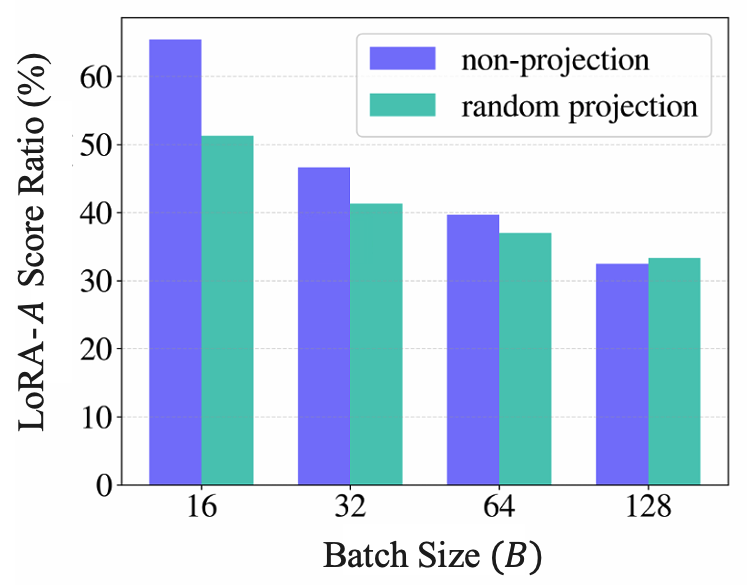
\includegraphics[width=0.4\linewidth]{figures/6_experiments/ablation_rp.png}
\caption{Comparison of LoRA-A score ratio with and without random projection across different batch sizes.}
\label{fig:ablation_rp_score}
\end{figure}

To examine whether the benefit of random projection is related to channel-wise 
gradient outliers, we vary the batch size in DP-SGD, since larger batches can 
average stochastic gradient fluctuations and reduce the effect of outliers.
As shown in Table~\ref{tab:ablation_rp}, the performance gap between Proposed 
and Proposed w/o RP decreases as the batch size increases.
At $B{=}32$, random projection improves QQP accuracy by 2.03 pp, while the improvement reduces to 0.79 pp at $B{=}128$.
This trend suggests that random projection is particularly effective when smaller 
batch sizes make channel-wise outliers less likely to be canceled through batch 
averaging.
As the batch size increases and this implicit averaging effect becomes stronger, 
the additional benefit of random projection becomes smaller.
% ---------- top-right table ----------
\begin{wraptable}{r}{0.45\linewidth}
\vspace{3pt}
\centering
\scriptsize
\setlength{\tabcolsep}{2pt}
\renewcommand{\arraystretch}{1.05}
\newcommand{\std}[1]{\,{\tiny$\pm$}\,\tiny #1}

\caption{Comparison with/without random projection under DP-SGD ($\epsilon=6$).}
\label{tab:ablation_rp}
\begin{tabular}{lccc}
\toprule
\textbf{Method} & QQP ($B$=32) & QQP ($B$=64) & QQP ($B$=128) \\
\midrule
Proposed
& $\textbf{63.19}$\std{0.01}
& $\textbf{73.99}$\std{1.41}
& $\textbf{79.94}$\std{0.11}\\

Proposed w/o RP
& 61.16\std{2.03}
& 70.90\std{2.78}
& 79.15\std{0.69}\\
\bottomrule
\end{tabular}

\vspace{-10pt}
\end{wraptable}

Figure~\ref{fig:ablation_rp_score} further corroborates this interpretation by 
visualizing the LoRA-$A$ score ratio across different batch sizes.
At small batch sizes (e.g., $B{=}16$), the LoRA-$A$ score ratio under 
non-projection is substantially higher than that under random projection, 
indicating that channel-wise outliers inflate the $A$ component's score and 
cause it to be disproportionately favored in mode selection.
As the batch size increases, the gap between non-projection and random projection 
narrows steadily, and at $B{=}128$ the two nearly coincide.
This confirms that larger batches implicitly suppress outlier effects through 
averaging, reducing the discrepancy between the two scoring strategies.
Taken together, these results support that the proposed random projection 
effectively mitigates channel-wise gradient outliers and leads to more balanced 
and reliable score estimation, particularly in the small-batch regime typical of 
DP-SGD training.



\begin{wraptable}{r}{0.44\linewidth}
\vspace{-13pt}
\centering
\scriptsize
\setlength{\tabcolsep}{2pt}
\renewcommand{\arraystretch}{1.05}
\newcommand{\std}[1]{\,{\tiny$\pm$}\,\tiny #1}

\caption{Comparison of single-pass and two-pass under DP-SGD ($\epsilon=3$).}
\label{tab:pass}

\begin{tabular}{lcc}
\toprule
\textbf{Method} & \textbf{MNLI (m)} & \textbf{MNLI (mm)} \\
\midrule
single-pass (ours)
& 79.15\std{0.23}
& 80.03\std{0.30} \\

two-pass inner-loop computation
& 79.37\std{0.31}
& 80.29\std{0.26} \\
\bottomrule
\end{tabular}

\vspace{-8pt}
\end{wraptable}

\subsection{Single-Pass vs. Two-Pass Score Computation}
\label{app:pass}

We compare two designs for score computation that differ in when and how the 
scores are evaluated relative to the communication rounds.

In the \emph{single-pass} design (ours), each client computes the scores as a 
by-product of local training and uploads them to the server together with the 
updated LoRA parameters.
The server then maintains EMA-smoothed scores across rounds and uses them to 
determine the mode vector for the \emph{next} round, requiring no additional 
communication beyond the standard parameter exchange.
As a result, the mode selection at round $t$ is based on historically smoothed 
scores rather than the current global model state.

In the \emph{two-pass inner-loop} design, the server first broadcasts both the 
$A$ and $B$ components of the current global model to all clients.
Each client then evaluates the scores for both components locally and sends them 
back to the server.
The server aggregates the received scores and determines the mode vector based 
on the current global model, after which the selected components are redistributed 
to the clients for local training.
This design enables greedy, round-wise mode selection based on the most 
up-to-date global model state, at the cost of an additional communication round 
and extra local computation per round.

As shown in Table~\ref{tab:pass}, the two-pass inner-loop computation achieves 
slightly higher performance than the single-pass design, improving MNLI~(m) and 
MNLI~(mm) by $+0.22$ and $+0.26$ pp, respectively.
However, the performance gap is marginal, and the single-pass design avoids the 
additional communication and computation overhead introduced by the two-pass 
approach.
These results demonstrate that the single-pass design provides a favorable 
trade-off between performance and efficiency.


\begin{wraptable}{r}{0.39\linewidth}
\vspace{-13pt}
\centering
\scriptsize
\setlength{\tabcolsep}{2pt}
\renewcommand{\arraystretch}{1.05}
\newcommand{\std}[1]{\,{\tiny$\pm$}\,\tiny #1}

\caption{Comparison of mode selection rules. Experiments are conducted under DP-SGD ($\epsilon=6$) with $B=64$.}
\label{tab:mode_selection_ablation}

\begin{tabular}{lcc}
\toprule
\textbf{Mode Selection Strategy}
& \textbf{MNLI (m)}
& \textbf{MNLI (mm)} \\
\midrule

Majority voting
& \textbf{75.56}\std{1.51}
& 76.31\std{2.38} \\

Weighted averaging
& 75.50\std{1.58}
& \textbf{76.60}\std{1.97} \\


Ours (Uniform averaging)
& 74.48\std{0.04}
& 75.15\std{0.35} \\

\bottomrule
\end{tabular}
\end{wraptable}
\subsection{Effect of aggregation rule}  \label{app:selection_rule}
We further study alternative rules for aggregating layer-wise mode decisions across clients. 
Specifically, we consider three variants: (i) \textit{majority voting}, where each client independently selects its preferred mode and the server adopts the mode receiving the majority of votes;
(ii) \textit{weighted averaging}, which computes a data-size weighted average of client scores before selecting a mode; and 
(iii) \textit{uniform averaging} (ours), which averages client scores uniformly and determines the mode accordingly.
As shown in Table~\ref{tab:mode_selection_ablation}, majority voting and weighted averaging achieve higher performance than uniform averaging on both MNLI (m) and MNLI (mm), suggesting that the aggregation rule for mode selection can meaningfully affect the quality of the selected modes. We adopt uniform averaging as the default aggregation strategy throughout this paper. Even with this simple aggregation, AS-LoRA outperforms 
prior federated LoRA methods; further gains are expected when combined 
with more sophisticated aggregation rules including majority rule, weighted aggregation.


\begin{figure*}[h]
\centering
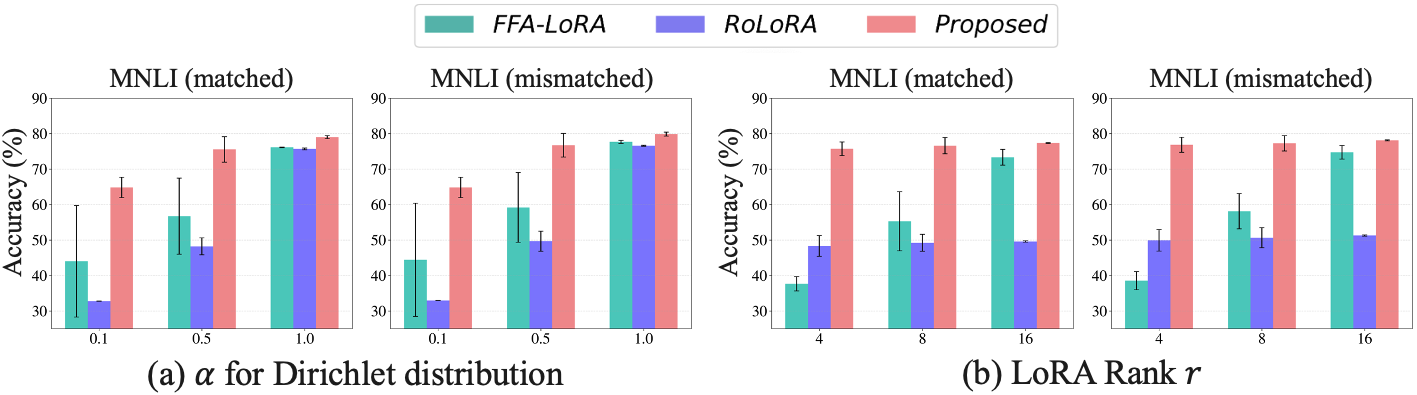
\includegraphics[width=1.0\textwidth]{figures/6_experiments/analysis_alpha_r.png}
\caption{(a): Comparison under varying dirichlet distribution $\alpha \in \{0.1,0.5,1.0\}$ on the MNLI dataset. (b): Comparison under varying LoRA rank $r \in \{4,8,16\}$ on the MNLI dataset. The number of clients is fixed at $K=3$ under DP-SGD ($\epsilon=6$).}
\label{fig:analysis_alpha_r}
\end{figure*}
\subsection{Effect of LoRA rank and data distribution} \label{app:alpha_rank}
In Figure~\ref{fig:analysis_alpha_r}(a), the proposed method consistently achieves the best performance across all $\alpha$ values and shows larger gains at smaller $\alpha$. This suggests stronger robustness under highly heterogeneous settings. The advantage of the proposed method is maintained across all heterogeneity levels.
In Figure~\ref{fig:analysis_alpha_r}(b), performance generally improves as the LoRA rank increases. The proposed method consistently outperforms the baselines across all rank settings and maintains its advantage even at low ranks. Notably, the performance improvement of FFA-LoRA is more pronounced than that of RoLoRA as the rank increases, suggesting that FFA-LoRA benefits more from the increased expressive capacity provided by larger ranks.


\subsection{Communication and memory overhead analysis} \label{app:communication_overhead}
We analyze the additional overhead introduced by AS-LoRA. Let $\mathcal{M}_n$
denote the set of LoRA modules in Transformer layer $n$. We define
\[
P_A=\sum_{n=1}^{N}\sum_{m\in\mathcal{M}_n} r d_{\mathrm{in},m}(n),
\qquad
P_B=\sum_{n=1}^{N}\sum_{m\in\mathcal{M}_n} r d_{\mathrm{out},m}(n),
\]
where $P_A$ and $P_B$ denote the number of trainable parameters in the $A$ and
$B$ LoRA components, respectively. FedLoRA communicates $P_A+P_B$ parameters
per client per round, whereas FFA-LoRA communicates $P_B$, and RoLoRA
communicates either $P_A$ or $P_B$. AS-LoRA also communicates only one active
component per layer and therefore has the same order of parameter communication
as alternating methods.

The additional communication of AS-LoRA comes only from the score and mode
information. In our implementation, all LoRA modules within the same Transformer
layer share one layer-level mode decision. Thus, each client uploads two scalar
scores per Transformer layer, and the server broadcasts one binary mode
indicator per layer. The additional uplink and downlink costs are therefore
$N$ floating-point values and $N$ bits per round, respectively. For a 24-layer
backbone, this corresponds to only $24$ FP32 values, or $96$ bytes, per client
per round, which is less than $0.02\%$ of the active LoRA parameter
communication when the hidden dimension is 1024.
\subsection{Computational overhead analysis}  \label{app:computational_overhead}

We analyze the computational overhead of the proposed curvature-based 
scoring and present practical strategies to overcome it.
We note that $\|\tilde{g}\|^2$ is obtained as a byproduct of the 
standard backward pass and incurs no additional computation.

\textbf{FLOPs accounting.}
Following~\cite{kaplan2020scaling}, we set $C_{\mathrm{bwd}} \approx 2C_{\mathrm{fwd}}$, 
so one local update step costs $3C_{\mathrm{fwd}}$.
Over $T=100$ rounds with $\tau=10$ local steps, the baseline FLOPs are:
\[
\mathcal{F}_{\mathrm{base}} = 3\tau T = 3 \times 10 \times 100 = 3{,}000\;C_{\mathrm{fwd}}.
\]
The proposed method uses a central-difference FD scheme requiring 
two forward passes per scoring target per round.
With $N_{\mathrm{target}} = 24$ targets (one active component per layer), 
the full per-round curvature scoring costs:
\[
\mathcal{F}_{\mathrm{full}} = N_{\mathrm{target}} \times 2 \times T
= 24 \times 2 \times 100 = 4{,}800\;C_{\mathrm{fwd}},
\]
yielding an overhead of $4{,}800 / 3{,}000 = \mathbf{160\%}$ over the baseline,
which is prohibitive for resource-constrained deployments.

We propose two complementary strategies to reduce this overhead.
First, replacing the central-difference scheme with a one-sided scheme:
\[
c_{a,k}^t(n) \approx 
\frac{\mathcal{L}_k^t(W_t + \epsilon_{\mathrm{fd}}\,v_{a,k}^t(n)) 
- \mathcal{L}_k^t(W_t)}{\epsilon_{\mathrm{fd}}^2},
\]
halves the per-target cost by reusing $\mathcal{L}_k^t(W_t)$ 
already computed during training.
Second, applying curvature scoring only every $f$ rounds reduces 
the number of scoring events from $T$ to $T/f$.
Under both strategies with $f=10$, the curvature overhead becomes:
\[
\mathcal{F}_{\mathrm{curv}} = N_{\mathrm{target}} \times 1 \times \frac{T}{f}
= 24 \times 10 = 240\;C_{\mathrm{fwd}},
\]
reducing the overhead to $240 / 3{,}000 \approx \mathbf{8\%}$---a 
$20\times$ reduction from the original $160\%$.

\begin{wraptable}{r}{0.34\textwidth}
\vspace{-13pt}
\centering
\scriptsize
\setlength{\tabcolsep}{2pt}
\renewcommand{\arraystretch}{1.05}
\newcommand{\std}[1]{\,{\tiny$\pm$}\,\tiny #1}
\caption{
    Comparison of curvature computation schedules in AS-LoRA under DP-SGD ($\epsilon=3$).
}
\label{app:scheduling}
\begin{tabular}{lcc}
\toprule
\textbf{Method} & \textbf{MNLI (m)} & \textbf{MNLI (mm)} \\
\midrule
\multicolumn{3}{l}{\textit{Periodic computation}} \\
($f{=}5$)   & 77.99\std{1.17} & 79.39\std{1.07} \\
($f{=}10$)  & 78.83\std{1.08} & 79.76\std{0.80} \\
\midrule
\multicolumn{3}{l}{\textit{Late-phase computation}} \\
($T^*{=}80$) & 78.91\std{1.11} & 79.87\std{0.95} \\
($T^*{=}90$) & 78.85\std{0.88} & \textbf{80.11}\std{0.74} \\
\midrule
\multicolumn{3}{l}{\textit{Original}} \\
Proposed (ours) & \textbf{79.15}\std{0.23} & 80.03\std{0.40} \\
\bottomrule
\end{tabular}
\vspace{-3pt}
\end{wraptable}

\textbf{Scheduling strategies.}
We consider two scheduling variants:
\textbf{(i) Periodic}: compute curvature scores every $f \in \{5, 10\}$ 
rounds and use $\|\tilde{g}\|^2$ otherwise.
\textbf{(ii) Late-phase}: apply $\|\tilde{g}\|^2$ for the first 
$T^* \in \{80, 90\}$ rounds and switch to curvature scoring thereafter, 
motivated by the observation that $\|\tilde{g}\|^2$ dominates early 
optimization while $g_a^\top H_a g_a$ becomes informative as 
$\|\tilde{g}\|^2$ diminishes near convergence.


\textbf{Analysis.}
As shown in Table~\ref{app:scheduling}, late-phase scheduling 
($T^*{=}80$) incurs only $-0.24$ degradation on MNLI (m) 
relative to the full method.
Notably, $T^*{=}90$ surpasses the full method on MNLI (mm) 
while reducing overhead from $160\%$ to $8\%$ ($20\times$ reduction).
These results confirm that full per-round curvature scoring is unnecessary: 
selective scheduling preserves most of the performance gain 
at a fraction of the computational cost.



\begin{wraptable}{r}{0.39\linewidth}
\vspace{-13pt}
\centering
\scriptsize
\setlength{\tabcolsep}{2pt}
\renewcommand{\arraystretch}{1.05}
\newcommand{\std}[1]{\,{\tiny$\pm$}\,\tiny #1}

\caption{Effect of gradient smoothing methods under DP-SGD ($\epsilon=3$).}
\label{tab:smoothing}

\begin{tabular}{lcc}
\toprule
\textbf{Method} & \textbf{MNLI (m)} & \textbf{MNLI (mm)} \\
\midrule
Proposed (w/o smoothing)
& 79.15\std{0.23}
& 80.03\std{0.40} \\

Gaussian
& 78.85\std{0.14}
& 79.74\std{0.21} \\

Laplacian
& \textbf{79.48}\std{0.16}
& \textbf{80.31}\std{0.16} \\

EMA
& 77.70\std{0.19}
& 78.65\std{0.14} \\
\bottomrule
\end{tabular}

\vspace{-8pt}
\end{wraptable}

\subsection{Effect of gradient smoothing under DP-SGD}\label{app:kernel}
We investigate whether applying smoothing to DP-SGD gradients can further improve utility, motivated by the observation that injected Gaussian noise in DP-SGD is high-frequency in nature and may be partially mitigated by frequency-selective filtering. Specifically, we compare three smoothing strategies applied to the aggregated gradients: (i) a standard 5-tap Gaussian filter $[1/16,\,4/16,\,6/16,\,4/16,\,1/16]$ as proposed in~\cite{liu2026rethinking}, (ii) Laplacian smoothing~\cite{liang2024differentially}, and (iii) EMA across communication rounds

The Gaussian noise injected by DP-SGD is i.i.d.\ across parameters and thus behaves as white noise in the parameter space, concentrating its energy uniformly across all frequencies.In contrast, the true gradient signal is typically smooth and sparse in the frequency domain, with energy concentrated at low frequencies.In the frequency domain, Laplacian smoothing acts as:
\begin{equation}
    \hat{g}_{\mathrm{smooth}}(\omega) 
    = \frac{\hat{g}(\omega)}{1 + \sigma \lambda(\omega)},
    \label{eq:laplacian_freq}
\end{equation}
where $\lambda(\omega)$ denotes the eigenvalue of the graph Laplacian at frequency $\omega$ and $\sigma > 0$ is a smoothing coefficient.Since $\lambda(\omega) \approx 0$ for low frequencies, the true gradient signal passes through largely intact, whereas high-frequency noise components are strongly suppressed as $\lambda(\omega)$ grows. By contrast, the 5-tap Gaussian filter is a weighted average with fixed kernel $[1/16, 4/16, 6/16, 4/16, 1/16]$, which attenuates \emph{all} frequency components including low-frequency signal, leading to signal distortion. EMA operates along the time axis rather than the parameter space, and therefore cannot exploit the spatial structure of DP noise within a single round, making it the least compatible with the spatial nature of DP-SGD noise.

Table~\ref{tab:smoothing} reports the effect of each smoothing method under $\epsilon = 3$ on the MNLI matched (m) and mismatched (mm) benchmarks. The results are consistent with our frequency-domain analysis. Laplacian smoothing is the only method that improves over the no-smoothing baseline, gaining $+0.33$ and $+0.28$ pp on MNLI (m) and MNLI (mm), respectively.
Gaussian filtering slightly degrades performance relative to the baseline ($-0.30$ pp on MNLI (m)), confirming that indiscriminate attenuation of all frequency components distorts the gradient signal. EMA yields the largest degradation ($-1.45$ pp on MNLI (m)), as temporal averaging across rounds is ill-suited for suppressing within-round spatial noise introduced by DP-SGD. These findings suggest that frequency-selective smoothing, specifically Laplacian smoothing, is the most compatible post-processing strategy for DP-SGD gradients.



\subsection{Analysis of Layer-wise Mode Selection Patterns.} \label{app:mode_selection}

Figure~\ref{fig:mode_all} visualizes the layer-wise mode selection patterns over training rounds across different tasks, revealing several non-random and task-dependent behaviors. Overall, the proposed method does not produce uniformly alternating selections across layers; instead, each task exhibits its own characteristic layer-wise preference structure, indicating that the adaptive scores capture meaningful optimization differences between LoRA-$A$ and LoRA-$B$ components rather than inducing arbitrary switching behavior.

For language understanding tasks such as QNLI, MNLI, SST-2, QQP, and SNLI, mode selection patterns often exhibit partially coherent structures across neighboring layers. Certain intermediate or upper layers consistently favor the same component over many rounds, while other layers switch more frequently. This suggests that the relative utility of LoRA-$A$ and LoRA-$B$ varies across Transformer depth, with different layers playing distinct roles in private federated adaptation depending on both task and layer.

In contrast, vision tasks exhibit more mixed and fine-grained switching. On CIFAR-100 and Tiny-ImageNet, selected modes distribute more evenly across layers and rounds, with fewer large contiguous regions dominated by a single component. This implies that in vision tasks, the relative advantage between LoRA-$A$ and LoRA-$B$ varies more locally across rounds, leading to less stable layer-wise specialization than in language tasks.

These observations have two key implications. First, they support the need for adaptive layer-wise mode selection, as a fixed global schedule cannot capture such heterogeneous preferences across tasks and layers. Second, recurring structures in language tasks suggest cross-layer dependencies not explicitly modeled by the current greedy formulation. Although each AS-LoRA layer independently selects its active component based on its score, the dynamics imply that groups of layers may prefer similar modes or evolve in a correlated manner over training rounds.

This also highlights a limitation of the current framework. Our analysis and algorithm focus on layer-wise greedy selection, enabling tractable optimization and strong empirical performance, but do not exploit inter-layer correlations. Future work could extend AS-LoRA to a joint decision framework that models structured dependencies across layers, for example by encouraging coordinated mode assignments among related layers or learning higher-level scheduling policies over layer groups. Such extensions may improve global coordination and yield more efficient update schedules beyond the current independent layer-wise strategy.

\begin{figure}[t]
    \centering

    % Row 1
    \begin{subfigure}{0.48\linewidth}
        \centering
        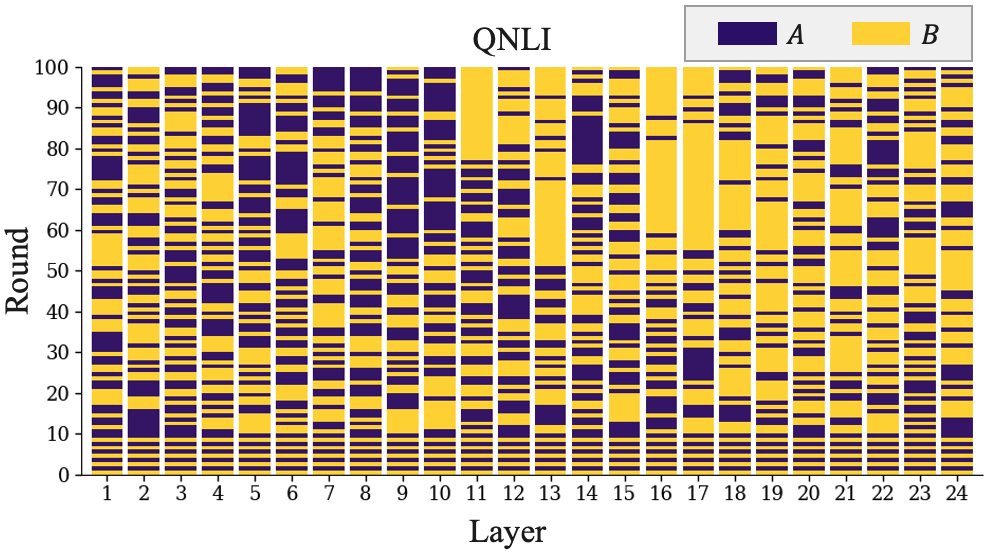
\includegraphics[width=\linewidth]{./figures/8_appendix/mode_qnli.png}
        \caption{QNLI}
    \end{subfigure}
    \hfill
    \begin{subfigure}{0.48\linewidth}
        \centering
        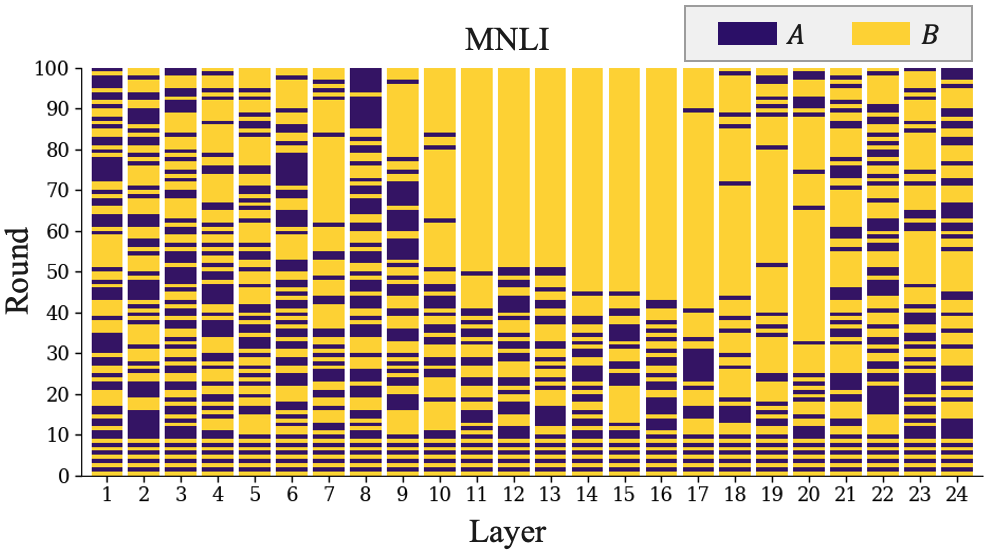
\includegraphics[width=\linewidth]{./figures/8_appendix/mode_mnli.png}
        \caption{MNLI}
    \end{subfigure}

    \vspace{6pt}

    % Row 2
    \begin{subfigure}{0.48\linewidth}
        \centering
        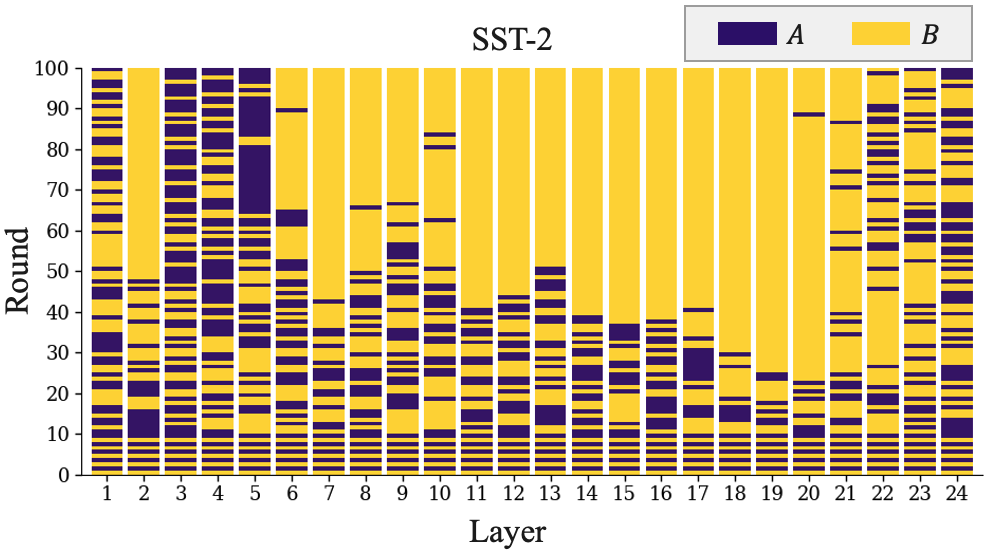
\includegraphics[width=\linewidth]{./figures/8_appendix/mode_sst2.png}
        \caption{SST-2}
    \end{subfigure}
    \hfill
    \begin{subfigure}{0.48\linewidth}
        \centering
        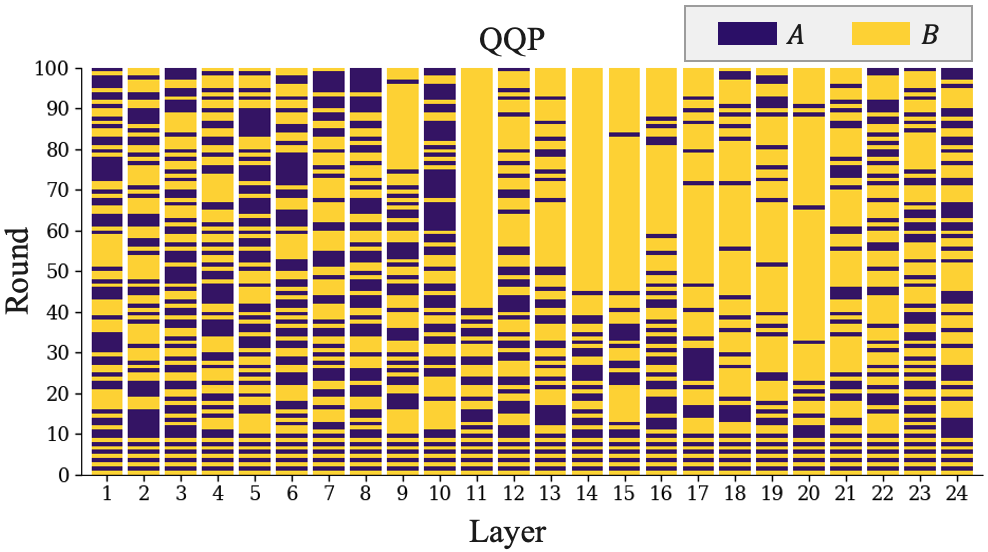
\includegraphics[width=\linewidth]{./figures/8_appendix/mode_qqp.png}
        \caption{QQP}
    \end{subfigure}

    \vspace{6pt}

    % Row 3
    \begin{subfigure}{0.48\linewidth}
        \centering
        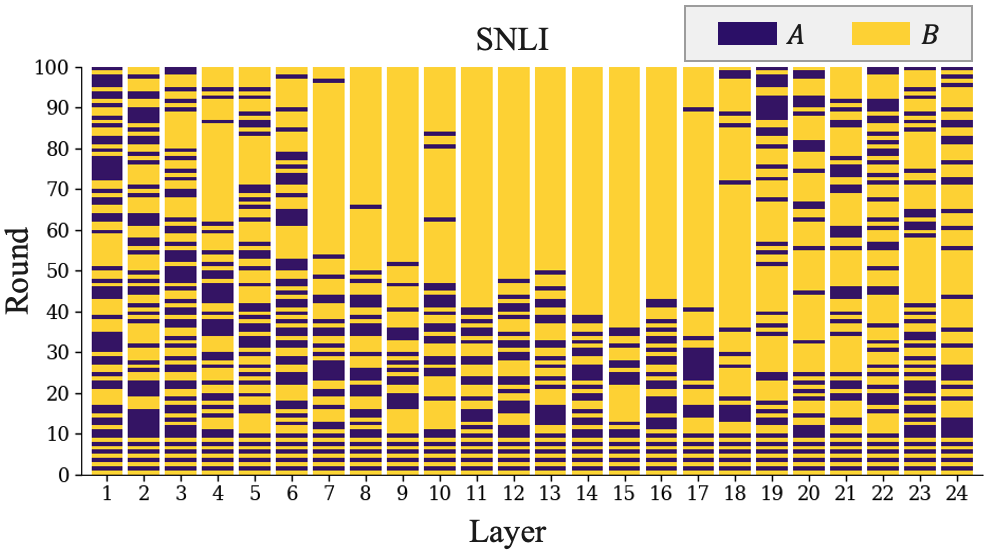
\includegraphics[width=\linewidth]{./figures/8_appendix/mode_snli.png}
        \caption{SNLI}
    \end{subfigure}
    \hfill
    \begin{subfigure}{0.48\linewidth}
        \centering
        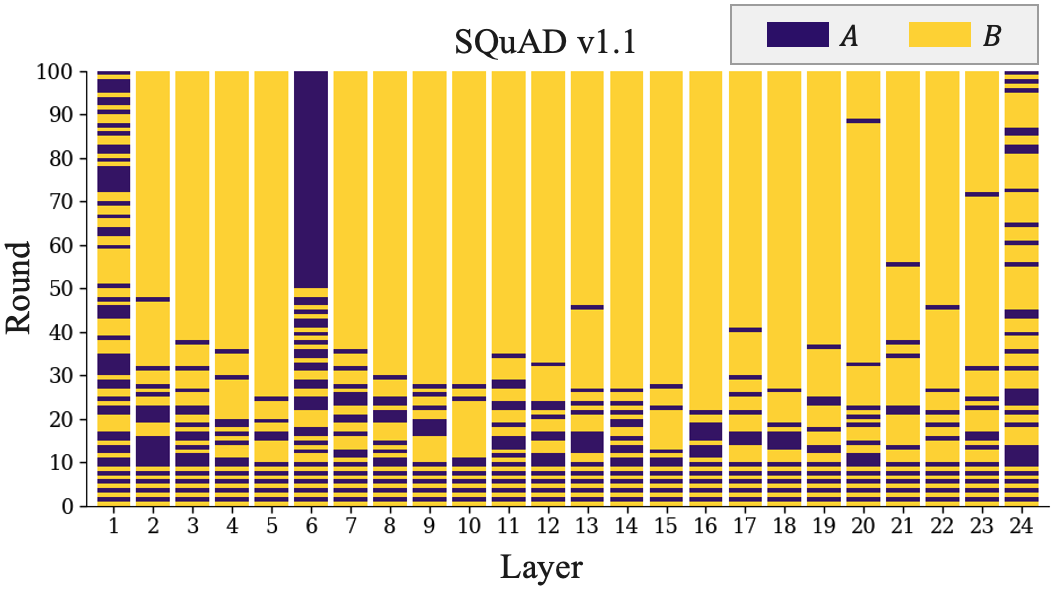
\includegraphics[width=\linewidth]{./figures/8_appendix/mode_squad11.png}
        \caption{SQuAD v1.1}
    \end{subfigure}

    \vspace{6pt}

    % Row 4 (추가)
    \begin{subfigure}{0.48\linewidth}
        \centering
        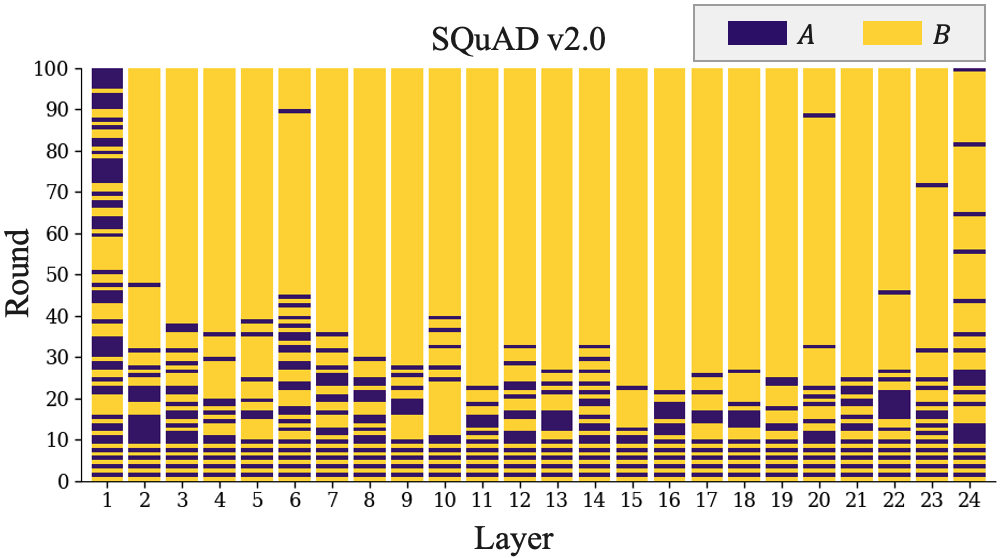
\includegraphics[width=\linewidth]{./figures/8_appendix/mode_squad20.png}
        \caption{SQuAD v2.0}
    \end{subfigure}
    \hfill
    \begin{subfigure}{0.48\linewidth}
        \centering
        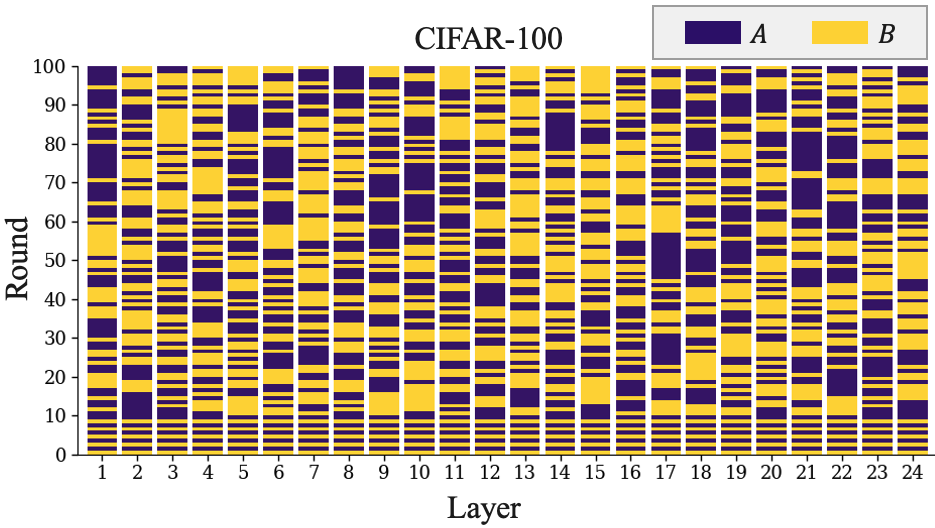
\includegraphics[width=\linewidth]{./figures/8_appendix/mode_cifar100.png}
        \caption{CIFAR-100}
    \end{subfigure}

    \vspace{6pt}

    % Row 5 (마지막 1개 가운데 정렬)
    \begin{subfigure}{0.48\linewidth}
        \centering
        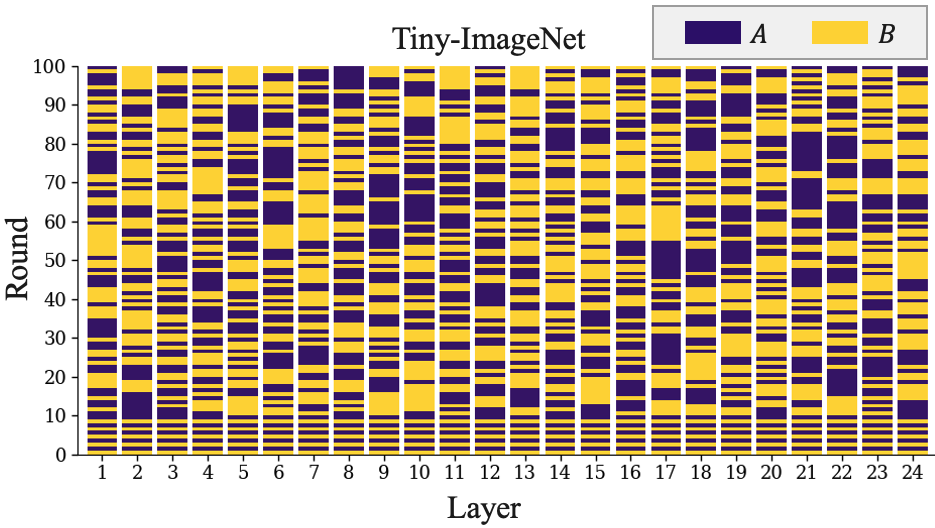
\includegraphics[width=\linewidth]{./figures/8_appendix/mode_tiny.png}
        \caption{Tiny-ImageNet}
    \end{subfigure}

    \caption{Layer-wise mode selection patterns across different tasks.}
    \label{fig:mode_all}
\end{figure}

